% main.tex — Comportamiento del Consumidor Digital: Datos, Perfiles y Modelos
% Libro de texto y manual de laboratorio · Dr. Aboud Barsekh-Onji
% IPN — ESCA Unidad Santo Tomás · Licenciatura en Mercadotecnia Digital

\documentclass[11pt,letterpaper]{book}
% preamble.tex — Comportamiento del Consumidor Digital: Datos, Perfiles y Modelos
% Dr. Aboud Barsekh-Onji · IPN — ESCA Unidad Santo Tomás

\usepackage[utf8]{inputenc}
\usepackage[T1]{fontenc}
\usepackage[spanish,es-noindentfirst]{babel}
% El atajo activo " de babel-spanish (usado para guillemets "< "> y otras
% combinaciones) rompe las comillas rectas normales dentro de una palabra
% (p. ej. "esto?" seguido de una letra genera basura tipográfica). Se
% desactiva y se usa \enquote{} de csquotes para comillas en todo el libro.
\shorthandoff{"}
\usepackage{csquotes}
\usepackage[letterpaper,margin=2.5cm,headheight=14pt]{geometry}

\usepackage{amsmath,amssymb}
\usepackage{booktabs}
\usepackage{graphicx}
\usepackage{hyperref}
\usepackage{fancyhdr}
\usepackage{tikz}
\usetikzlibrary{arrows.meta,positioning,shapes.geometric}
\usepackage{pgfplots}
\pgfplotsset{compat=1.18}
\usepackage{microtype}
\usepackage{todonotes}
\usepackage{enumitem}
\usepackage{caption}
\usepackage{capt-of} % \captionof{figure}{...} para figuras no flotantes dentro de tcolorbox (recuadros de Laboratorio)

% Paleta y macros (deben cargarse antes que macros.tex por las cajas tcolorbox)
% config/colores.tex — paleta institucional y semántica del libro
% Fase 1 (D1.2): HEX oficial tomado del skill `beamer-ipn` (Manual de Identidad
% Gráfica del IPN, Pantone 222C), confirmado por el Dr. Barsekh-Onji — sustituye
% la aproximación provisional de Fase 0.
\usepackage[dvipsnames,svgnames,x11names]{xcolor}

% --- Paleta institucional IPN (idéntica a beamer-ipn, para reutilizar figuras
% entre el libro y las presentaciones de la Fase 5, §14 del prompt) ---
\definecolor{guindaIPN}{HTML}{6F1D46}       % Pantone 222C oficial — color primario
\definecolor{guindaIPNOsc}{HTML}{45102C}    % sombra / secundario
\definecolor{guindaIPNClara}{HTML}{F4E9EF}  % fondo de bloques normales
\definecolor{doradoIPN}{HTML}{B8975A}       % SOLO enlaces y detalles, nunca fondo de bloque
\definecolor{terracotaIPN}{HTML}{9C5B44}    % bloques de advertencia/atención
\definecolor{terracotaIPNClara}{HTML}{F6ECE6}
\definecolor{bronceIPN}{HTML}{8C6B3F}       % bloques de ejemplo
\definecolor{bronceIPNClaro}{HTML}{F5F0E3}
\definecolor{grisIPN}{HTML}{58595B}         % texto secundario / notas

% --- Paleta funcional del libro (recuadros, listados, gráficas) ---
% Mapeo alineado a la convención beamer-ipn (block=guinda, alertblock=terracota,
% exampleblock=bronce); Frontera y Laboratorio son propios del libro (no existen
% como bloque en las slides) y usan acentos que no compiten con esos tres.
\colorlet{colorDefinicion}{guindaIPN}
\colorlet{colorEjemplo}{bronceIPN}
\colorlet{colorAtencion}{terracotaIPN}
\colorlet{colorFrontera}{doradoIPN}   % acento dorado como borde de "novedad" (nunca como fondo de bloque)
\colorlet{colorEtica}{guindaIPNOsc}   % guinda oscuro: distinto de Atención (terracota) y Frontera (dorado)
\definecolor{colorLaboratorio}{HTML}{1B6E7A} % teal técnico: distingue el laboratorio MATLAB de la identidad institucional

% Paleta de código (listings) — sintaxis ESTÁNDAR del lenguaje, nunca
% recoloreada al guinda institucional (misma regla que beamer-ipn, §"Código")
\definecolor{codeblue}{rgb}{0,0,1}
\definecolor{codegreen}{rgb}{0,0.6,0}
\definecolor{codegray}{HTML}{58595B}
\definecolor{codepurple}{rgb}{0.5,0,0.5}
\definecolor{codebg}{rgb}{0.97,0.97,0.99}

% config/macros.tex — macros de trazabilidad y recuadros del libro

% --- Trazabilidad contra el programa oficial (§4) ---
% Uso: \progtag{1.1.1} coloca una etiqueta \label{prog:1.1.1} invisible en el margen,
% usada por el script de verificación de cobertura (docs/cobertura.md).
\newcommand{\progtag}[1]{\label{prog:#1}}

% --- Marcadores de pendientes (§5.2, §9) — visibles en el PDF y listados aparte ---
\newcommand{\pendiente}[1]{%
  \textcolor{colorAtencion}{\textbf{[PENDIENTE: #1]}}%
}
\newcommand{\datoPendiente}[1]{%
  \textcolor{colorAtencion}{\textbf{[DATO PENDIENTE DE VERIFICAR: #1]}}%
}

% --- Recuadros tcolorbox (§11) ---
\usepackage[most]{tcolorbox}
\tcbuselibrary{skins,breakable}

\newtcolorbox{cajaDefinicion}[1][]{%
  colback=colorDefinicion!5, colframe=colorDefinicion, breakable,
  fonttitle=\bfseries, title={Definición}, #1}

\newtcolorbox{cajaEjemplo}[1][]{%
  colback=colorEjemplo!5, colframe=colorEjemplo, breakable,
  fonttitle=\bfseries, title={Ejemplo}, #1}

\newtcolorbox{cajaAtencion}[1][]{%
  colback=colorAtencion!5, colframe=colorAtencion, breakable,
  fonttitle=\bfseries, title={Atención}, #1}

\newtcolorbox{cajaFrontera}[1][]{%
  colback=colorFrontera!5, colframe=colorFrontera, breakable,
  fonttitle=\bfseries, title={Frontera}, #1}

\newtcolorbox{cajaEtica}[1][]{%
  colback=colorEtica!5, colframe=colorEtica, breakable,
  fonttitle=\bfseries, title={Ética y responsabilidad con los datos}, #1}

\newtcolorbox{cajaLaboratorio}[1][]{%
  colback=colorLaboratorio!5, colframe=colorLaboratorio, breakable,
  fonttitle=\bfseries, title={Laboratorio MATLAB}, #1}

% Ficha del capítulo (§8.1): recuadro neutro, administrativo — no compite
% visualmente con los recuadros de contenido (Definición, Frontera, Ética...).
\newtcolorbox{cajaFicha}[1][]{%
  colback=grisIPN!6, colframe=grisIPN, breakable, sharp corners,
  boxrule=0.6pt, left=8pt, right=8pt, top=4pt, bottom=4pt,
  fonttitle=\bfseries, title={Ficha del capítulo}, #1}

% --- Vigencia de temas selectos (§5.7) ---
\newcommand{\vigente}[1]{\textit{(Vigente a #1)}}

% --- Caso ilustrativo ficticio (§5.6) ---
\newenvironment{casoFicticio}{%
  \begin{cajaEjemplo}[title={Caso ilustrativo (ficticio)}]%
}{%
  \end{cajaEjemplo}%
}

% config/listings-matlab.tex — estilo de código para MATLAB y Python
\usepackage{listings}

\lstdefinestyle{MATLABStyle}{
  language=Matlab,
  backgroundcolor=\color{codebg},
  basicstyle=\ttfamily\small,
  keywordstyle=\color{codeblue}\bfseries,
  commentstyle=\color{codegreen}\itshape,
  stringstyle=\color{codepurple},
  numbers=left,
  numberstyle=\tiny\color{codegray},
  numbersep=8pt,
  frame=single,
  rulecolor=\color{codegray!40},
  breaklines=true,
  showstringspaces=false,
  tabsize=2,
  captionpos=b,
}

\lstdefinestyle{PythonStyle}{
  language=Python,
  backgroundcolor=\color{codebg},
  basicstyle=\ttfamily\small,
  keywordstyle=\color{codeblue}\bfseries,
  commentstyle=\color{codegreen}\itshape,
  stringstyle=\color{codepurple},
  numbers=left,
  numberstyle=\tiny\color{codegray},
  numbersep=8pt,
  frame=single,
  rulecolor=\color{codegray!40},
  breaklines=true,
  showstringspaces=false,
  tabsize=4,
  captionpos=b,
}

\lstset{style=MATLABStyle}


% --- Citación: APA 7.ª ed. con biblatex + biber (§5.4 del prompt de proyecto).
% Corrección de Fase 0/1: biblatex-apa SÍ está instalado (paquete Debian
% texlive-bibtex-extra); la comprobación inicial con kpsewhich buscó un
% archivo "biblatex-apa.sty" que no existe con ese nombre — el paquete se
% activa vía style=apa (apa.bbx/apa.cbx/apa.dbx), no con \usepackage{biblatex-apa}.
\usepackage[backend=biber,style=apa,language=spanish,uniquename=false]{biblatex}
\addbibresource{bib/referencias.bib}

% --- Glosario ---
\usepackage[acronym,toc]{glossaries}
\makeglossaries

% --- Encabezados ---
\pagestyle{fancy}
\fancyhf{}
\fancyhead[LE,RO]{\thepage}
\fancyhead[RE]{\nouppercase{\leftmark}}
\fancyhead[LO]{\nouppercase{\rightmark}}
\renewcommand{\headrulewidth}{0.4pt}

\hypersetup{
  colorlinks=true,
  linkcolor=guindaIPN,
  citecolor=colorDefinicion,
  urlcolor=colorDefinicion,
  pdftitle={Comportamiento del Consumidor Digital: Datos, Perfiles y Modelos},
  pdfauthor={Aboud Barsekh-Onji}
}


\begin{document}

% frontmatter/portada.tex
\begin{titlepage}
\centering
{\scshape\large Instituto Politécnico Nacional\par}
\vspace{0.2cm}
{\large Escuela Superior de Comercio y Administración, Unidad Santo Tomás\par}
\vspace{0.2cm}
{\large Licenciatura en Mercadotecnia Digital\par}
\vspace{2cm}
{\Huge\bfseries Comportamiento del Consumidor Digital\par}
\vspace{0.4cm}
{\Large Datos, Perfiles y Modelos\par}
\vspace{0.6cm}
{\large\itshape Libro de texto y manual de laboratorio\par}
\vspace{0.4cm}
{\normalsize Laboratorio: Gestión de datos, comportamiento y perfiles del consumidor digital \\ 3.\textsuperscript{er} semestre\par}
\vfill
{\large Dr. Aboud Barsekh-Onji\par}
\vspace{0.5cm}
{\normalsize \today\par}
\end{titlepage}

\frontmatter
\tableofcontents
% frontmatter/mapa-cobertura.tex
% Mapa de cobertura del programa oficial -> capítulos del libro.
% Fuente completa y actualizable (interna, no citada al lector): docs/cobertura.md.

\chapter*{Mapa de cobertura del programa oficial}
\addcontentsline{toc}{chapter}{Mapa de cobertura del programa oficial}

Esta tabla resume la correspondencia entre las cinco unidades temáticas del
programa oficial \textit{Laboratorio: Gestión de datos, comportamiento y
perfiles del consumidor digital} (IPN-ESCA Santo Tomás, vigente desde agosto de
2022) y los capítulos de este libro. El programa oficial completo, con sus 66
subtemas, se cubre íntegramente a lo largo de los 18 capítulos.

\begin{table}[htbp]
\centering
\begin{tabular}{@{}clc@{}}
\toprule
Unidad & Título & Capítulos \\
\midrule
I   & Comportamiento, perfil y gestión de datos & 1--4 \\
II  & Proceso de toma de decisión de compra digital & 5--8 \\
III & Modelos de comportamiento del consumidor digital & 9--12 \\
IV  & Factores socioculturales y psicológicos & 13--16 \\
V   & Análisis integral del comportamiento del consumidor digital & 17--18 \\
\bottomrule
\end{tabular}
\caption{Mapa de cobertura por unidad. Fuente: elaboración propia a partir del
programa oficial de la unidad de aprendizaje, IPN-ESCA Unidad Santo Tomás.}
\label{tab:mapa-cobertura}
\end{table}

\pendiente{Completar este mapa con el detalle subtema por subtema al cerrar
cada Parte del libro.}


\mainmatter
% --- Capítulo de prueba de Fase 0: retirado en Fase 2 (docs/pendientes.md) ---
% % frontmatter/capitulo-prueba.tex
% Capítulo de PRUEBA de Fase 0 — verifica el flujo completo: recuadro tcolorbox,
% figura TikZ, figura MATLAB exportada y una cita bibliográfica (natbib+apalike).
% No forma parte del libro final; se sustituye por el Cap. 1 real en la Fase 2.

\chapter*{Capítulo de prueba (verificación de andamiaje, Fase 0)}
\addcontentsline{toc}{chapter}{Capítulo de prueba (verificación de andamiaje)}
\progtag{0.0.0}

Este capítulo existe únicamente para verificar, antes de escribir contenido real,
que el flujo \texttt{MATLAB → figura vectorial → \LaTeX{}} y los elementos
tipográficos definidos en \texttt{config/} compilan sin errores.

\begin{cajaDefinicion}
El \textit{customer journey} (recorrido del consumidor) es la secuencia de puntos
de contacto que un consumidor atraviesa desde el reconocimiento de una necesidad
hasta la evaluación posterior a la compra \parencite{solomon2017}.
\end{cajaDefinicion}

\begin{figure}[htbp]
  \centering
  % figuras/tikz/fase0-diagrama-prueba.tex
% Diagrama de prueba (Fase 0): tres etapas simples del recorrido del consumidor.
% Compilable solo (standalone) o incluible con \input en el libro/Beamer.
\begin{tikzpicture}[
    etapa/.style={rectangle, rounded corners, draw=guindaIPN, thick,
                  fill=guindaIPN!8, minimum width=3.1cm, minimum height=1.1cm,
                  align=center, font=\small},
    flecha/.style={-{Stealth[length=2.5mm]}, thick, draw=doradoIPN}
  ]
  \node[etapa] (a) {Reconocimiento\\ de necesidad};
  \node[etapa, right=1.6cm of a] (b) {Búsqueda de\\ información};
  \node[etapa, right=1.6cm of b] (c) {Evaluación\\ posterior};

  \draw[flecha] (a) -- (b);
  \draw[flecha] (b) -- (c);
\end{tikzpicture}

  \caption{Diagrama conceptual de prueba (TikZ). Fuente: elaboración propia.}
  \label{fig:fase0-tikz}
\end{figure}

\begin{figure}[htbp]
  \centering
  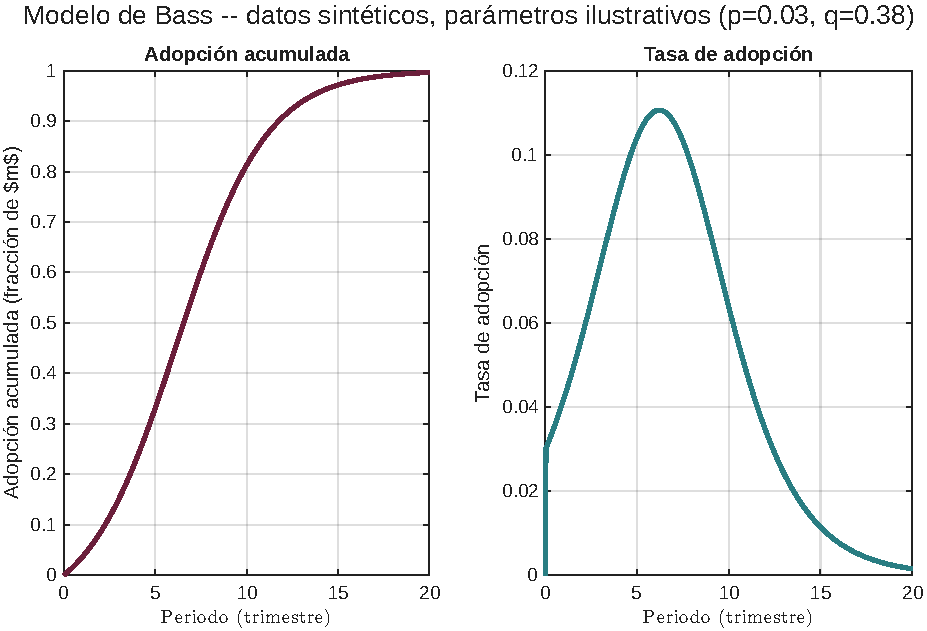
\includegraphics[width=0.9\textwidth]{figuras/matlab/fase0_bass_prueba.pdf}
  \caption{Curva de adopción del modelo de Bass. Fuente: elaboración propia con
  datos sintéticos, \texttt{rng(42)}, parámetros ilustrativos.}
  \label{fig:fase0-matlab}
\end{figure}

\begin{cajaEtica}
Toda cifra de mercado que aparezca en el libro final estará respaldada en
\texttt{docs/verificacion-datos.md}; los datos de esta figura son sintéticos y
están rotulados como tales, conforme al \S5.8 del prompt de proyecto.
\end{cajaEtica}

\pendiente{Sustituir este capítulo por el contenido real del Cap. 1 en la Fase 2.}


% --- PARTE I — Comportamiento, perfil y gestión de datos (Fase 2) ---
% partes/parte1/intro.tex
\part{Comportamiento, perfil y gestión de datos}

\chapter*{Introducción a la Parte I}
\addcontentsline{toc}{chapter}{Introducción a la Parte I}

Un mismo clic significa cosas distintas según quién lo interprete. Para el
consumidor, es el cierre de una decisión: comparó, dudó, se decidió. Para la
plataforma que registró ese clic, es un dato entre millones, destinado a
alimentar un modelo que predice el próximo clic de alguien más. Esta Parte
trata sobre esa doble naturaleza del consumo digital: es, a la vez, una
experiencia vivida por una persona y un rastro estructurado que una
organización puede analizar, agregar y usar para decidir.

El programa oficial de la unidad llama a esta Parte \enquote{Comportamiento, perfil y
gestión de datos del consumidor digital}, y su competencia es identificar la
evolución del consumidor digital a partir de sus tipos de perfil y de la
gestión de los datos que genera. Cuatro capítulos la desarrollan. El primero
sitúa históricamente al consumidor digital: qué cambió, qué no, y por qué
conviene desconfiar de las periodizaciones ordenadas en versiones (\enquote{del
consumidor 1.0 al 5.0}) que la literatura de consultoría presenta como si
fueran hechos científicos. El segundo aborda el perfil y la segmentación:
cómo se agrupa a los consumidores, y por qué la pertenencia rígida a un solo
segmento es, en muchos mercados, una simplificación conveniente más que una
descripción fiel del comportamiento real. El tercero entra en la gestión de
datos propiamente dicha: cómo se crea valor a partir de ellos, qué significa
\enquote{escuchar} a un consumidor digital, y qué obligaciones legales y éticas trae
consigo recolectar esa información en México en 2026. El cuarto cierra con la
base tecnológica que hace posible todo lo anterior: buscadores, plataformas,
redes sociales y comercio electrónico, tratados no como un catálogo de marcas
sino como un conjunto de criterios de análisis que sobrevivan al cambio de
esas marcas.

Un hilo conecta los cuatro capítulos: la gestión de datos del consumidor
digital no es neutral. Cada decisión de qué medir, cómo segmentar y qué
inferir tiene consecuencias sobre la privacidad, la autonomía y, en última
instancia, la confianza del consumidor en la organización que lo observa. Por
eso cada capítulo cierra con un recuadro de ética y responsabilidad con los
datos: no como formalidad, sino porque la pregunta \enquote{¿debería medirse esto?}
es tan parte del oficio del mercadólogo digital como la pregunta \enquote{¿cómo se
mide esto?}.

Las prácticas oficiales de esta Parte —\enquote{El consumidor digital y su perfil} y
\enquote{Buscadores y plataformas en la gestión de datos del consumidor digital}— se
integran en las secciones de laboratorio de cada capítulo y se consolidan al
final de la Parte, en la sección \enquote{Prácticas oficiales de la unidad}.

% partes/parte1/cap01.tex
\chapter{El consumidor digital: evolución, impacto y ventajas de su análisis}
\label{cap:01}

\begin{cajaFicha}
\begin{description}
  \item[Unidad temática] I — Comportamiento, perfil y gestión de datos del consumidor digital.
  \item[Temas del programa] 1.1 Comportamiento del consumidor: 1.1.1 Evolución del consumidor 1.0 al 5.0 y tendencias a futuro; 1.1.2 Impacto del consumo digital inteligente y sostenible; 1.1.3 Ventajas del análisis del comportamiento del consumidor digital.
  \item[Horas] Teoría 2.0 · Práctica 4.0 · Aprendizaje autónomo 2.0.
  \item[Competencia de la unidad] Identifica el comportamiento del consumidor digital y su evolución a partir de sus tipos de perfil y gestión de datos.
  \item[Resultados de aprendizaje observables] Al concluir el capítulo, el estudiante:
  \begin{enumerate}
    \item distingue la evolución real del consumidor digital de su periodización comercial en \enquote{versiones};
    \item explica, con al menos dos fuentes verificables, qué significa consumo digital inteligente y sostenible en el contexto mexicano;
    \item argumenta, con datos, al menos tres ventajas concretas de analizar el comportamiento del consumidor digital para una organización.
  \end{enumerate}
  \item[Prerrequisitos] Ninguno formal; se recomienda familiaridad básica con conceptos de mercadotecnia general (mezcla de mercadotecnia, segmentación elemental).
\end{description}
\end{cajaFicha}

\section{Caso de apertura}

En 2015, el 57.4\,\% de la población mexicana de seis años o más usaba
internet. Diez años después, en 2025, esa cifra llegó a 86.1\,\%
\parencite{inegi2026endutih}. En el mismo periodo, el comercio electrónico
pasó de ser una curiosidad urbana a mover 941 mil millones de pesos anuales,
con 77.2 millones de compradores digitales \parencite{amvo2026}. Ninguna de
las dos cifras describe una revolución instantánea. Describen una curva:
lenta al principio, acelerada después, hoy cercana a su techo natural en
ciertos segmentos de la población y todavía lejos de él en otros (compárese
el 86.9\,\% de penetración urbana contra el 68.5\,\% rural en 2024;
\parencite{inegi2025endutih}). Este capítulo empieza ahí, con la pregunta que
suele saltarse en los diagnósticos de mercadotecnia: ¿la evolución del
consumidor digital es un fenómeno que se puede medir con esa curva, o es,
además, una narrativa que ciertas editoriales de consultoría han sabido
vender en entregas sucesivas? Las dos cosas son ciertas, y distinguirlas es
el primer ejercicio de rigor analítico que pide este libro.

\section{Desarrollo teórico}

\subsection{Evolución del consumidor: de la curva de adopción a la narrativa de versiones}
\progtag{1.1.1}

Dos relatos compiten para explicar cómo cambió el consumidor en las últimas
tres décadas. El primero es empírico: mide penetración de internet, uso de
dispositivos, volumen de transacciones digitales. El segundo es editorial:
organiza el cambio en versiones numeradas, del 1.0 al 6.0, cada una con un
librito que la anuncia. Conviene no confundirlos.

La serie \textit{Marketing X.0}, de Philip Kotler, Hermawan Kartajaya e Iwan
Setiawan, es el origen del segundo relato. \textit{Marketing 3.0} (2010)
proponía un giro hacia los valores del consumidor; \textit{Marketing 4.0}
(2016/2017), hacia la integración de lo digital y lo presencial;
\textit{Marketing 5.0} (2021), hacia la tecnología aplicada al factor humano
\parencite{kotler2021marketing50}; \textit{Marketing 6.0} (2024), hacia la
inmersión —internet de las cosas, inteligencia artificial, realidad
aumentada— bajo la etiqueta de \enquote{metamarketing} \parencite{kotler2024marketing6}.
La figura~\ref{fig:cap01-lineamx0} muestra esta secuencia.

\begin{figure}[htbp]
  \centering
  % figuras/tikz/cap01-linea-marketing-x0.tex
% Línea de tiempo crítica: la serie "Marketing X.0" de Kotler, Kartajaya y Setiawan
% como periodización editorial (no modelo académico validado empíricamente).
\begin{tikzpicture}[
    hito/.style={rectangle, rounded corners, draw=guindaIPN, thick, fill=guindaIPNClara,
                 minimum width=2.6cm, minimum height=1.4cm, align=center, font=\footnotesize},
    linea/.style={thick, draw=grisIPN}
  ]
  \draw[linea, -{Stealth[length=3mm]}] (-0.3,0) -- (13.3,0);

  \node[hito] (m1) at (0,0.9) {\textbf{1.0}\\[1pt] Producto\\ (s.\,f.)};
  \node[hito] (m2) at (3.3,0.9) {\textbf{2.0}\\[1pt] Consumidor\\ (s.\,f.)};
  \node[hito] (m3) at (6.6,0.9) {\textbf{3.0}\\[1pt] Valores\\ 2010};
  \node[hito] (m4) at (9.9,0.9) {\textbf{4.0}\\[1pt] Digital\\ 2016};
  \node[hito] (m5) at (13.2,0.9) {\textbf{5.0}\\[1pt] Tecnología\\ 2021};

  \foreach \x in {0,3.3,6.6,9.9,13.2} {
    \draw[linea] (\x,0) -- (\x,0.2);
  }

  \node[hito, fill=bronceIPNClaro, draw=bronceIPN] (m6) at (13.2,-1.3) {\textbf{6.0}\\[1pt] Inmersivo\\ 2024};
  \draw[linea] (13.2,-0.2) -- (13.2,-0.6);

  \node[align=center, font=\scriptsize\itshape, text width=13.5cm] at (6.5,-2.6)
    {Serie editorial de libros (Kotler, Kartajaya y Setiawan), no un programa de\\
     investigación arbitrado: cada entrega se alinea a la tecnología dominante de su año de publicación.};
\end{tikzpicture}

  \caption{La serie \enquote{Marketing X.0} como periodización editorial. Cada
  entrega se publica alineada a la tecnología dominante de su momento; no es
  un programa de investigación con aparato empírico propio ni revisión por
  pares. Fuente: elaboración propia con base en
  \parencite{kotler2021marketing50,kotler2024marketing6}.}
  \label{fig:cap01-lineamx0}
\end{figure}

Cada entrega de la serie es útil como lectura de tendencias de la práctica
profesional. Ninguna es, en el sentido estricto, un modelo académico
validado: no hay una teoría del consumidor 4.0 sometida a revisión por pares
con la misma exigencia metodológica que, por ejemplo, la teoría de la
segmentación de mercado de Wendell Smith, publicada casi setenta años antes
en el \textit{Journal of Marketing} \parencite{smith1956}. Esta distinción no
resta valor a la serie de Kotler et al. como diagnóstico de industria. Sí
exige presentarla con el estatus que le corresponde: una lectura influyente
de consultoría, no un hecho histórico objetivo. El libro más reciente sobre
comportamiento del consumidor digital que localizamos, de Jagdish Sheth y
Varsha Jain \parencite{sheth2026}, evita la lógica de versiones y organiza el
cambio por mecanismos —qué datos genera el consumidor, cómo se procesan, qué
decisiones habilitan— en vez de por eras. Es un contraste metodológico que
vale la pena señalar al estudiante: hay más de una forma legítima de narrar
el mismo cambio.

¿Qué cambió entonces, de forma verificable? Tres cosas, con evidencia
directa: la proporción de la población con acceso a internet (evidencia en
\S\ref{sec:cap01-evidencia}), el tipo de decisiones que se toman en entornos
digitales en vez de presenciales, y la cantidad de rastro de datos que cada
decisión deja disponible para el análisis. Este último punto es el que abre
el resto del libro: no es solo que el consumidor cambió, es que ahora se
puede observar de una manera que antes no existía.

Esa posibilidad de observación introduce la tensión de fondo que recorre
todo el libro: el consumidor digital tiene una doble naturaleza, es persona
vivida y es, simultáneamente, dato estructurado disponible para el análisis
(figura~\ref{fig:cap01-doble-naturaleza}). Ninguna de las dos lecturas basta
por sí sola —una organización que solo ve datos pierde el contexto humano de
la decisión; una que solo ve personas no puede operar a la escala que exige
un mercado digital de millones de usuarios—, y sostener las dos en tensión,
sin colapsar en ninguna, es la competencia central que este libro busca
desarrollar.

\begin{figure}[htbp]
  \centering
  % figuras/tikz/cap01-doble-naturaleza.tex
% Diagrama conceptual: el consumidor digital como persona vivida y como dato
% estructurado — las dos lecturas que el capítulo pide distinguir.
\begin{tikzpicture}[
    caja/.style={rectangle, rounded corners, draw=guindaIPN, thick, fill=guindaIPNClara,
                 minimum width=5cm, minimum height=2.6cm, align=center, font=\small},
    etiqueta/.style={font=\scriptsize\itshape, text width=5cm, align=center},
    flecha/.style={-{Stealth[length=2.5mm]}, thick, draw=doradoIPN}
  ]
  \node[caja] (persona) at (0,0) {\textbf{Consumidor}\\ como persona\\[4pt]
    necesidad, deseo,\\ contexto, emoción};
  \node[caja] (dato) at (7,0) {\textbf{Consumidor}\\ como dato\\[4pt]
    clic, sesión, patrón,\\ variable de un modelo};

  \draw[flecha] (persona) -- node[above, font=\scriptsize, align=center] {se registra\\ como} (dato);
  \draw[flecha] (dato) to[bend left=25] node[below, font=\scriptsize] {predice y moldea} (persona);

  \node[etiqueta] at (0,-1.9) {Unidad de análisis: la experiencia individual};
  \node[etiqueta] at (7,-1.9) {Unidad de análisis: el agregado estadístico};
\end{tikzpicture}

  \caption{El consumidor digital como persona vivida y como dato
  estructurado: dos unidades de análisis en tensión permanente. Fuente:
  elaboración propia.}
  \label{fig:cap01-doble-naturaleza}
\end{figure}

\subsection{Impacto del consumo digital inteligente y sostenible}
\progtag{1.1.2}

\enquote{Consumo inteligente} y \enquote{consumo sostenible} no son sinónimos, aunque el
discurso de mercadotecnia digital tiende a fusionarlos. El primero se refiere
a decisiones de compra informadas por datos y comparación (uso de
comparadores de precio, lectura de reseñas, verificación de especificaciones
técnicas antes de comprar). El segundo se refiere al impacto ambiental y
social de esas decisiones, con independencia de qué tan informadas estén.

En México, PROFECO ha incorporado explícitamente el lenguaje de la economía
circular en su comunicación al consumidor: la Revista del Consumidor dedicó
en septiembre de 2025 un número a la vida útil de los dispositivos
electrónicos y a la compra de productos remanufacturados, con el objetivo
declarado de evitar el \textit{greenwashing} —reclamos ambientales que no se
pueden verificar— mediante etiquetado responsable
\parencite{profeco2025entornodigital}. El marco internacional de referencia
es el Objetivo de Desarrollo Sostenible 12 de la ONU, Producción y Consumo
Responsables \parencite{onu2015ods12}, que sitúa el consumo digital dentro de
un problema más amplio: la producción de dispositivos, servidores y
conectividad tiene un costo ambiental que la conversación de mercadotecnia
digital, centrada casi siempre en la conversión y la retención, tiende a dejar
fuera del análisis.

\begin{cajaFrontera}
\textbf{Consumo sostenible: la brecha entre actitud y conducta.}
Que un consumidor declare preferencia por productos sostenibles no significa
que los compre. La literatura académica llama a esto \textit{brecha
actitud-conducta} (\textit{attitude-behavior gap}): la actitud pro-ambiental
autoinformada predice, de forma sistemática, peor la conducta de compra real
de lo que predeciría un modelo de conducta planeada bien especificado —entran
en juego el precio relativo, la conveniencia percibida y la confianza en que
la etiqueta ambiental sea cierta. No localizamos, al cierre de esta
investigación, un estudio con cifras específicas de esta brecha para el
mercado mexicano: es una oportunidad de indagación documental legítima para
el portafolio de evidencias de este capítulo, no un hueco que debamos llenar
con una cifra sin verificar.
\end{cajaFrontera}

\subsection{Ventajas del análisis del comportamiento del consumidor digital}
\progtag{1.1.3}

¿Para qué le sirve a una organización analizar sistemáticamente el
comportamiento de su consumidor digital, más allá de la intuición del
equipo de mercadotecnia? El cuadro~\ref{tab:cap01-ventajas} resume cuatro
ventajas con distinto nivel de evidencia, deliberadamente clasificadas para
que el estudiante distinga la que está bien establecida en la literatura de
la que es, todavía, promesa de proveedor de tecnología.

\begin{table}[htbp]
\centering
\begin{tabular}{@{}p{3.2cm}p{6.3cm}p{3.5cm}@{}}
\toprule
Ventaja & Descripción & Nivel de evidencia \\
\midrule
Segmentación más precisa & Agrupar consumidores por comportamiento observado, no solo por variables demográficas declaradas & Alto — literatura arbitrada desde Smith (1956) \\
Personalización de la oferta & Ajustar producto, precio o mensaje al perfil inferido del consumidor & Medio — efectividad documentada, pero con límites (fatiga de personalización, percepción de vigilancia) \\
Reducción de fricción en el recorrido & Detectar en qué punto del proceso de decisión abandona el consumidor y corregirlo & Alto — instrumentable directamente con analítica de embudo \\
Anticipación de tendencias & Detectar cambios de comportamiento antes que la competencia & Bajo-medio — depende de la calidad y representatividad del dato, riesgo de sobreajuste a ruido \\
\bottomrule
\end{tabular}
\caption{Ventajas del análisis del comportamiento del consumidor digital,
clasificadas por nivel de evidencia. Fuente: elaboración propia con base en
\parencite{smith1956,solomon2017,sheth2026}.}
\label{tab:cap01-ventajas}
\end{table}

La cuarta fila merece una advertencia explícita. \enquote{Anticipar tendencias} es la
promesa más común del discurso comercial de analítica de consumidor y la
menos sostenida por evidencia sistemática: un patrón detectado en datos
históricos no garantiza que se repita, y la literatura de economía
conductual documenta cómo los propios analistas caen en el sesgo de
representatividad al proyectar continuidad donde solo hubo una coincidencia
\parencite{tverskykahneman1974}. Este es el primer contacto del libro con un
tema que reaparecerá en los capítulos 5 y 10--11: los datos no eliminan el
sesgo humano en la toma de decisiones, lo pueden amplificar si no se
interpretan con criterio.

\section{Evidencia de México y del mundo}
\label{sec:cap01-evidencia}

\begin{table}[htbp]
\centering
\begin{tabular}{@{}lrr@{}}
\toprule
Indicador & 2024 & 2025 \\
\midrule
Población de 6+ años que usa internet & 83.1\,\% & 86.1\,\% \\
Adopción de internet, zona urbana & 86.9\,\% & — \\
Adopción de internet, zona rural & 68.5\,\% & — \\
Compradores digitales en México & — & 77.2 millones \\
Valor del comercio electrónico (crecimiento anual) & — & \$941{,}000 mdp (+19.2\,\%) \\
\bottomrule
\end{tabular}
\caption{Evolución reciente del consumidor digital en México. Fuente:
elaboración propia con datos de INEGI, ENDUTIH 2024 y 2025
\parencite{inegi2025endutih,inegi2026endutih}, y AMVO, Estudio de Venta
Online 2026 \parencite{amvo2026}.}
\label{tab:cap01-evidencia}
\end{table}

Dos lecturas se desprenden del cuadro~\ref{tab:cap01-evidencia}. La primera:
el crecimiento de la conectividad en México no se ha detenido, pero tampoco
es parejo —la brecha urbano-rural de dieciocho puntos porcentuales en 2024 es
más relevante para la práctica profesional que la cifra nacional agregada,
porque delimita en qué proporción del país una estrategia \enquote{todo digital} es
viable sin canales complementarios. La segunda: el crecimiento del comercio
electrónico (+19.2\,\% anual) supera al crecimiento de la conectividad
misma, lo que sugiere que buena parte del aumento no viene de gente nueva
conectándose, sino de gente ya conectada que compra más. Es una distinción
que el capítulo 3 retoma al hablar de toma de decisiones basadas en gestión
de datos.

\begin{cajaEtica}
Toda cifra de este capítulo proviene de fuente primaria verificable (INEGI,
AMVO) o está explícitamente marcada como estimación provisional. Ninguna
cifra de crecimiento o de tamaño de mercado citada en este libro se presenta
sin su fuente, año y fecha de consulta. Esto no es solo una norma editorial:
es el mismo estándar que el capítulo pide exigirle a cualquier proveedor de
analítica de consumidor que presente una cifra sin metodología pública.
Desconfiar de un dato no verificable es, en sí mismo, una competencia
profesional de mercadotecnia digital.
\end{cajaEtica}

\section{Laboratorio MATLAB: difusión de la adopción de un canal digital}

\begin{cajaLaboratorio}
\textbf{Objetivo.} Simular, con el modelo de Bass, cómo la proporción entre
adopción por innovación (decisión independiente) y adopción por imitación
(contagio social) cambia la forma de la curva de adopción de un canal
digital, e interpretar esa forma en términos de estrategia de lanzamiento.

\textbf{Concepto detrás del código.} El modelo de Bass \parencite{bass1969}
describe la tasa de adopción de una innovación como
\[
  \frac{dF(t)}{dt} = \big(p + q\,F(t)\big)\big(1 - F(t)\big),
\]
donde $F(t)$ es la fracción acumulada del mercado potencial que ya adoptó al
tiempo $t$, $p$ es el coeficiente de innovación y $q$ el de imitación. La
solución cerrada de esta ecuación diferencial,
\[
  F(t) = \frac{1 - e^{-(p+q)t}}{1 + \tfrac{q}{p}\,e^{-(p+q)t}},
\]
es la que implementa el script. El punto de inflexión de la curva —el
momento de máxima velocidad de adopción— ocurre en
$t^\ast = \ln(q/p)\,/\,(p+q)$: cuanto mayor es $q$ respecto a $p$, más tarde y
más abrupto es ese pico, porque la adopción depende más del contagio social
que de decisiones independientes.

\textbf{Script.} \texttt{matlab/cap01/cap01\_difusion\_bass.m}. Es el
\textbf{mismo script, sin modificar}, que se usa en la Práctica 1 de esta
Parte: toda la lógica de cálculo y graficación está fija; lo único que el
estudiante edita es el bloque de \textbf{parámetros}, claramente delimitado
al inicio del archivo. Corrida tal como está, usa parámetros
\textbf{didácticos} ($p=0.03$, $q=0.38$), no calibrados con datos reales de
un canal digital mexicano —decisión editorial deliberada, para mantener el
ejercicio enfocado en la forma de la curva y no en la calibración
estadística.

\begin{lstlisting}[style=MATLABStyle, caption={Bloque de parámetros editable (\texttt{cap01\_difusion\_bass.m}) — es lo único que cambia entre corridas.}]
p = 0.03;      % coeficiente de innovacion
q = 0.38;      % coeficiente de imitacion
m = 1;         % mercado potencial (normalizado)
tFinal = 20;   % periodos a simular
\end{lstlisting}

\textbf{Salida esperada.} Al correr el script (\texttt{Run}, sin editar nada
más que el bloque de parámetros) se imprimen en la ventana de comandos el
periodo del pico de adopción y el porcentaje de mercado adoptado al final del
periodo simulado, y se generan dos figuras: adopción acumulada
(figura~\ref{fig:cap01-bass-acum}) y tasa de adopción
(figura~\ref{fig:cap01-bass-tasa}), ambas con los valores de $p$ y $q$
usados en el título, para poder identificar de qué corrida viene cada una.

\begin{center}
  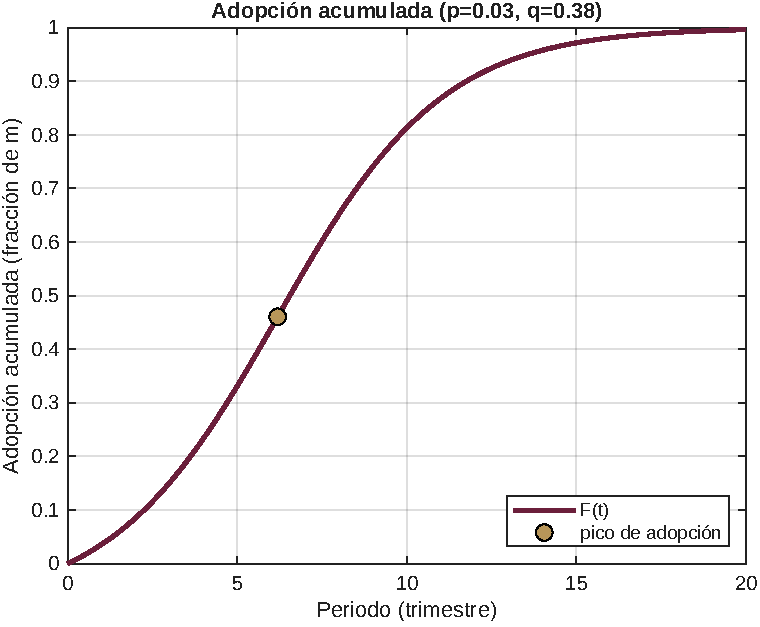
\includegraphics[width=0.75\textwidth]{figuras/matlab/cap01_bass_acumulada.pdf}
  \captionof{figure}{Adopción acumulada del modelo de Bass, parámetros
  didácticos ($p=0.03$, $q=0.38$). Fuente: elaboración propia con datos
  sintéticos, \texttt{rng(42)}.}
  \label{fig:cap01-bass-acum}
\end{center}

\begin{center}
  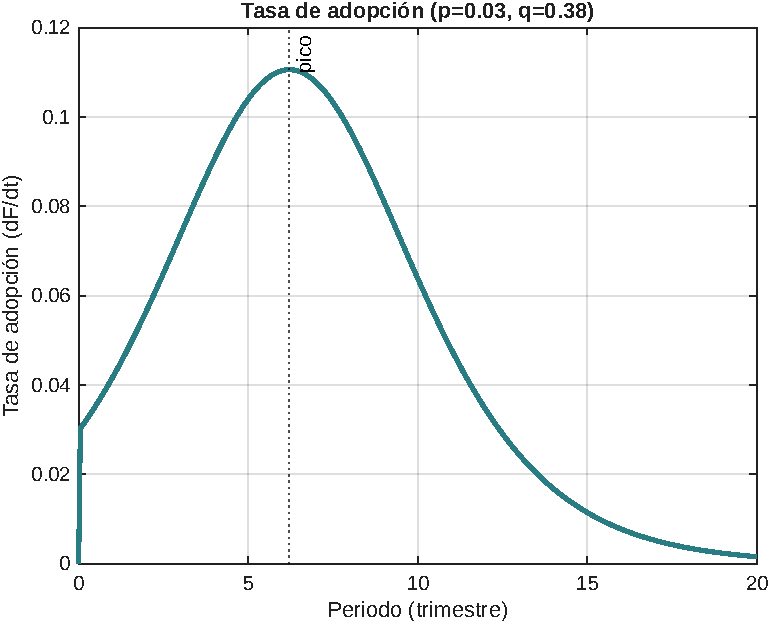
\includegraphics[width=0.75\textwidth]{figuras/matlab/cap01_bass_tasa.pdf}
  \captionof{figure}{Tasa de adopción del modelo de Bass, misma corrida.
  Fuente: elaboración propia con datos sintéticos.}
  \label{fig:cap01-bass-tasa}
\end{center}

\textbf{Interpretación de negocio.} El pico de esta corrida ($p=0.03$,
$q=0.38$) ocurre en $t^\ast \approx 6.2$ periodos, con 46\,\% del mercado ya
adoptado en ese momento. Cuanto mayor es $q$ respecto a $p$, más tarde y más
abrupto es ese pico —porque la adopción depende más del contagio social que
de decisiones independientes—, lo que en la figura se traduce en una fase
inicial más plana seguida de un despegue más pronunciado. El ejercicio
propuesto pide comprobar esto de primera mano, no como afirmación del libro.

\textbf{Ejercicio propuesto (usen exactamente este script, solo cambien el
bloque de parámetros).} Corran el script tres veces, una por caso, y
completen un cuadro con los resultados que imprime cada corrida:
\begin{enumerate}
  \item \textbf{Caso A — innovación dominante:} $p=0.08$, $q=0.10$.
  \item \textbf{Caso B — balance:} $p=0.03$, $q=0.38$ (los valores por defecto del script).
  \item \textbf{Caso C — imitación dominante:} $p=0.01$, $q=0.55$.
\end{enumerate}
Para cada caso, registren: el periodo del pico ($t^\ast$), el porcentaje de
mercado adoptado en ese pico, y el porcentaje de mercado adoptado al periodo
20. Con el cuadro completo, respondan por escrito: ¿en qué caso el pico
ocurre más tarde? ¿En qué caso la curva de adopción acumulada tiene una fase
inicial más plana? A partir de sus tres corridas —no de este libro—,
propongan un canal digital real (una app, una red social, un método de
pago) y justifiquen a cuál de los tres casos se parece más su patrón de
adopción esperado.

\textbf{Extensión opcional.} Investigar el modelo de Bass generalizado (con
coeficiente de presión de precio o de publicidad variable en el tiempo) y
describir, sin necesariamente programarlo, qué cambiaría en la forma de la
curva de este script.
\end{cajaLaboratorio}

\section{Estudio de caso}

\begin{casoFicticio}
Una fintech mexicana lanza una app de ahorro programado dirigida a
trabajadores independientes. A los tres meses del lanzamiento, la app tiene
2{,}000 usuarios activos —muy por debajo de la proyección inicial de 15{,}000—
y el equipo directivo discute si el producto \enquote{no funciona} o si simplemente
necesita más tiempo. El equipo de datos presenta dos lecturas alternativas de
la misma curva de adopción observada: una consistente con un canal dominado
por innovación (crecimiento lento pero sostenido, sin señales de contagio
entre usuarios), y otra consistente con un canal dominado por imitación
(la app apenas está saliendo del \enquote{valle} inicial y podría acelerar pronto si
el referido entre usuarios empieza a operar).

\textbf{Preguntas guía.}
\begin{enumerate}
  \item ¿Qué evidencia adicional —más allá del conteo de usuarios activos— permitiría distinguir entre las dos lecturas del caso?
  \item Si el diagnóstico correcto fuera \enquote{canal dominado por imitación en fase de valle}, ¿qué decisión de mercadotecnia sería la más riesgosa tomar en este momento?
  \item ¿Qué papel jugaría un programa de referidos en cambiar el balance entre $p$ y $q$ de este producto?
  \item Relacione este caso con la distinción entre \enquote{narrativa de versiones} y \enquote{evolución verificable} del \S 2.1: ¿qué tipo de evidencia usaría el equipo directivo para justificar su decisión frente a la dirección general, y por qué esa evidencia debe ser de fuente primaria?
\end{enumerate}
\end{casoFicticio}

\section{Actividades y evidencias del portafolio}

Alineadas con la estrategia oficial de la unidad (estudio de casos) y el
portafolio de evidencias de la Unidad I:

\begin{description}
  \item[Reporte de indagación documental] En equipos de tres a cuatro
  integrantes, investigar y contrastar dos fuentes académicas o
  institucionales (no blogs) sobre un concepto del capítulo no desarrollado
  en profundidad en el texto (p.\ ej., el marco de los cuatro niveles de la
  brecha digital, o el estado más reciente del comercio electrónico
  fronterizo). Criterio de evaluación: cada afirmación con cifra debe llevar
  fuente, año y fecha de consulta.
  \item[Exposición] Presentar en 8 minutos la comparación entre la
  \enquote{narrativa de versiones} (Marketing X.0) y la evolución verificable del
  consumidor digital mexicano, con al menos un dato de INEGI o AMVO no citado
  en este capítulo. Criterio de evaluación: distinción clara entre fuente
  primaria y lectura de consultoría.
  \item[Solución de casos] Resolver el estudio de caso de la fintech
  (\S 2.5) por escrito, con las cuatro preguntas guía respondidas y una
  recomendación final justificada.
  \item[Reporte de debate] En sesión plenaria, debatir la pregunta: \enquote{¿El
  consumo digital inteligente y el consumo sostenible son objetivos
  compatibles o están en tensión?}, con al menos una postura respaldada en la
  brecha actitud-conducta (recuadro de Frontera, \S 2.2).
  \item[Reporte de práctica] Entregar el cuadro de los tres casos del
  ejercicio propuesto del laboratorio (\S 3) —sin modificar el script, solo
  el bloque de parámetros— con las dos preguntas de comparación respondidas
  y la propuesta de canal digital real justificada.
\end{description}

\section{Ruta de aprendizaje autónomo}

Dos horas de aprendizaje autónomo asignadas a este capítulo. Tareas
concretas:
\begin{enumerate}
  \item Leer el comunicado de prensa más reciente de ENDUTIH (INEGI) y
  extraer tres cifras no citadas en este capítulo, con su fuente exacta.
  \item Revisar la ficha editorial de \textit{Marketing 6.0}
  \parencite{kotler2024marketing6} y anotar, en dos párrafos, si las
  tendencias que anuncia (inmersión, IA, IoT) ya son observables en algún
  servicio digital que el estudiante use cotidianamente.
  \item Ejecutar el script \texttt{cap01\_difusion\_bass.m} con los
  parámetros propios del ejercicio propuesto (\S 3) y anotar el tiempo del
  pico de adopción resultante.
\end{enumerate}

\section{Síntesis}

La evolución del consumidor digital admite dos lecturas que no deben
confundirse: una curva medible de adopción de tecnología y una narrativa
editorial organizada en versiones. Ambas son útiles; solo una es evidencia.
El consumo digital inteligente (decisiones informadas por datos) y el consumo
sostenible (decisiones con menor costo ambiental) son fenómenos distintos que
el discurso de mercadotecnia tiende a fusionar sin evidencia suficiente de
que coincidan en la práctica —la brecha actitud-conducta documenta
precisamente esa distancia. Analizar el comportamiento del consumidor digital
trae ventajas con niveles de evidencia desiguales: la segmentación basada en
comportamiento observado y la reducción de fricción en el recorrido de compra
están bien sustentadas; la anticipación de tendencias, la menos.

\subsection*{Glosario del capítulo}
\begin{description}
  \item[Brecha actitud-conducta] Distancia entre lo que un consumidor declara
  preferir y lo que efectivamente compra.
  \item[Consumo digital inteligente] Decisiones de compra informadas por
  datos y comparación en entornos digitales.
  \item[Coeficiente de imitación ($q$)] En el modelo de Bass, parámetro que
  mide cuánto depende la adopción del contagio social entre adoptantes.
  Rango matemático válido: $q \geq 0$ (sin cota superior estricta); en los
  casos didácticos de este libro se usan valores entre 0.10 y 0.55.
  \item[Coeficiente de innovación ($p$)] En el modelo de Bass, parámetro que
  mide la propensión a adoptar de forma independiente, sin influencia social.
  Rango matemático válido: $p > 0$ (si $p=0$, nadie inicia la adopción); en
  los casos didácticos de este libro se usan valores entre 0.01 y 0.08.
  \item[Mercado potencial ($m$)] En el modelo de Bass, tamaño del mercado
  objetivo, normalizado a 1 en este libro (equivale al 100\,\% del mercado).
  Rango: $m > 0$; con $m=1$, la adopción acumulada $F(t)$ queda expresada
  directamente como fracción del mercado.
  \item[\textit{Greenwashing}] Comunicación de atributos ambientales de un
  producto que no se pueden verificar o que exageran su impacto real.
\end{description}

\subsection*{Autoevaluación}

\textbf{Opción múltiple}

\begin{enumerate}
  \item La serie de libros \textit{Marketing X.0} (Kotler, Kartajaya y
  Setiawan) debe entenderse principalmente como:
  \begin{enumerate}
    \item[a)] Un programa de investigación académica revisado por pares.
    \item[b)] Una periodización editorial de consultoría alineada a la tecnología de cada momento. \textit{(correcta)}
    \item[c)] El primer marco teórico sobre comportamiento del consumidor digital.
    \item[d)] Una norma internacional de mercadotecnia digital.
  \end{enumerate}
  \textit{Justificación:} el capítulo documenta que cada entrega se publica
  alineada a la tecnología dominante de su año, sin aparato empírico propio
  ni revisión por pares (\S 2.1).

  \item En el modelo de Bass, si $q \gg p$, la curva de adopción se
  caracteriza por:
  \begin{enumerate}
    \item[a)] Crecimiento lineal y constante desde el inicio.
    \item[b)] Una fase inicial plana seguida de adopción explosiva. \textit{(correcta)}
    \item[c)] Adopción inmediata de todo el mercado potencial.
    \item[d)] Ausencia total de adopción.
  \end{enumerate}
  \textit{Justificación:} cuando la imitación domina, la adopción depende del
  contagio social, que requiere una base inicial de adoptantes antes de
  acelerar — comprobado en el ejercicio propuesto del \S 3 (Caso C).

  \item La brecha actitud-conducta en consumo sostenible se refiere a:
  \begin{enumerate}
    \item[a)] La diferencia de precio entre productos sostenibles y convencionales.
    \item[b)] La distancia entre la preferencia declarada y la compra real. \textit{(correcta)}
    \item[c)] La brecha digital rural-urbana.
    \item[d)] El costo ambiental de fabricar dispositivos electrónicos.
  \end{enumerate}
  \textit{Justificación:} ver recuadro de Frontera, \S 2.2.
\end{enumerate}

\textbf{Preguntas abiertas}

\begin{enumerate}
  \item Explique, con un ejemplo propio, por qué \enquote{consumo digital
  inteligente} y \enquote{consumo sostenible} no son sinónimos. \textit{Clave:} la
  respuesta debe distinguir la dimensión informacional (comparación,
  investigación previa) de la dimensión de impacto ambiental/social, y dar un
  ejemplo donde una decisión informada no sea, a la vez, sostenible (p.\ ej.,
  comparar precios para comprar más barato sin considerar huella de
  transporte).
  \item De las cuatro ventajas del análisis de comportamiento del consumidor
  digital presentadas en el cuadro~\ref{tab:cap01-ventajas}, elija la de
  menor nivel de evidencia y explique por qué. \textit{Clave:} la respuesta
  esperada es \enquote{anticipación de tendencias}, justificada por el riesgo de
  sobreajuste a patrones históricos que no se repiten y el sesgo de
  representatividad documentado por Tversky y Kahneman.
\end{enumerate}

\section{Lecturas recomendadas}

\begin{description}
  \item[\textcite{kotler2021marketing50}] Presenta el marco de las \enquote{5A} (Aware,
  Appeal, Ask, Act, Advocate) como evolución del embudo clásico. Útil para
  contrastar con la crítica al embudo lineal que desarrolla el capítulo 6 de
  este libro; leer con el mismo criterio crítico aplicado aquí a la serie
  Marketing X.0.
  \item[\textcite{sheth2026}] Organiza el comportamiento del consumidor digital
  por mecanismos de datos en vez de por eras cronológicas. Recomendado como
  contraste metodológico directo a la lógica de versiones.
  \item[\textcite{smith1956}] El artículo fundacional de la segmentación de
  mercado. Breve, denso, y la referencia obligada para entender de dónde
  viene el aparato conceptual que el capítulo 2 retoma con mayor detalle.
  \item[\textcite{onu2015ods12}] Página oficial del Objetivo de Desarrollo
  Sostenible 12. Punto de partida para el reporte de indagación documental
  sobre consumo sostenible.
\end{description}

% partes/parte1/cap02.tex
\chapter{Perfil, segmentación y mercado meta digital}
\label{cap:02}

\begin{cajaFicha}
\begin{description}
  \item[Unidad temática] I — Comportamiento, perfil y gestión de datos del consumidor digital.
  \item[Temas del programa] 1.2 Perfil del consumidor digital: 1.2.1 Segmentación del mercado digital y variables; 1.2.2 Mercado meta o target digital; 1.2.3 Tipos de perfil del consumidor digital; 1.2.4 Radiografía del consumidor digital en México y el mundo; 1.2.5 Diversidad de perfiles de consumidor digital por modelo de negocios-industria.
  \item[Horas] Teoría 2.0 · Práctica 3.0 · Aprendizaje autónomo 2.0.
  \item[Competencia de la unidad] Identifica el comportamiento del consumidor digital y su evolución a partir de sus tipos de perfil y gestión de datos.
  \item[Resultados de aprendizaje observables] Al concluir el capítulo, el estudiante:
  \begin{enumerate}
    \item aplica el proceso de segmentación-targeting-posicionamiento a un caso de mercado digital;
    \item distingue segmentación rígida de segmentación difusa y justifica cuándo cada una es preferible;
    \item describe, con datos verificados, la radiografía del consumidor digital mexicano frente al panorama internacional.
  \end{enumerate}
  \item[Prerrequisitos] Cap. 1 (evolución del consumidor digital).
\end{description}
\end{cajaFicha}

\section{Caso de apertura}

Una misma persona puede ser, para una plataforma de streaming, un
\enquote{usuario ocasional de fin de semana}, y para una app bancaria, un
\enquote{usuario de alto compromiso}. No hay contradicción: son dos negocios
midiendo comportamientos distintos sobre la misma persona. El error común de
la segmentación de manual es tratar al consumidor como si tuviera una sola
identidad de compra fija, aplicable a cualquier categoría. Este capítulo
propone lo contrario: el perfil de un consumidor digital es específico del
comportamiento que se mide, y —como se verá en el laboratorio— muchas veces
ni siquiera es una etiqueta única dentro de esa misma categoría.

\section{Desarrollo teórico}

\subsection{Segmentación del mercado digital y sus variables}
\progtag{1.2.1}

La segmentación de mercado tiene una fuente académica precisa: Wendell R.
Smith, quien en 1956 la definió, en contraste con la diferenciación de
producto, como la estrategia de \enquote{ver un mercado heterogéneo (...) como
un número de mercados homogéneos más pequeños, en respuesta a preferencias de
producto diferentes entre segmentos importantes del mercado}
\parencite{smith1956}. Sobre esa base se construyó, décadas después, el
proceso que hoy se enseña como estándar: Segmentación, Targeting y
Posicionamiento (STP), sistematizado en los manuales de Philip Kotler
\parencite{kotler2021marketing50}
(figura~\ref{fig:cap02-stp}).

\begin{figure}[htbp]
  \centering
  % figuras/tikz/cap02-stp.tex
% Proceso STP (Segmentación - Targeting - Posicionamiento), sistematización
% posterior construida sobre la base conceptual de Smith (1956).
\begin{tikzpicture}[
    etapa/.style={rectangle, rounded corners, draw=guindaIPN, thick, fill=guindaIPNClara,
                  minimum width=3.4cm, minimum height=1.6cm, align=center, font=\small},
    flecha/.style={-{Stealth[length=3mm]}, thick, draw=doradoIPN},
    nota/.style={font=\scriptsize, text width=3.4cm, align=center}
  ]
  \node[etapa] (s) at (0,0) {\textbf{Segmentación}\\ agrupar por\\ variables comunes};
  \node[etapa] (t) at (4.6,0) {\textbf{Targeting}\\ elegir el o los\\ segmentos meta};
  \node[etapa] (p) at (9.2,0) {\textbf{Posicionamiento}\\ definir el lugar\\ en la mente del\\ segmento meta};

  \draw[flecha] (s) -- (t);
  \draw[flecha] (t) -- (p);

  \node[nota] at (0,-1.4) {Smith (1956): base conceptual};
  \node[nota] at (4.6,-1.4) {Mercado meta o \textit{target}};
  \node[nota] at (9.2,-1.6) {Sistematización posterior (manuales de Kotler)};
\end{tikzpicture}

  \caption{El proceso STP como sistematización posterior de la base
  conceptual de Smith (1956). Fuente: elaboración propia.}
  \label{fig:cap02-stp}
\end{figure}

Las variables clásicas de segmentación —geográfica, demográfica,
psicográfica y conductual—, sistematizadas en la bibliografía de
comportamiento del consumidor \parencite{hoyer2024consumer}, no
desaparecieron con la digitalización; se
volvieron medibles con una granularidad que antes era impensable. El
cuadro~\ref{tab:cap02-variables} contrasta la versión analógica de cada
variable con su equivalente digital.

\begin{table}[htbp]
\centering
\begin{tabular}{@{}p{2.6cm}p{4.6cm}p{5.4cm}@{}}
\toprule
Variable & Versión clásica (encuesta/censo) & Equivalente digital (dato conductual) \\
\midrule
Geográfica & Región, ciudad declarada & Geolocalización de dispositivo, dirección IP, zona de entrega \\
Demográfica & Edad, sexo, ingreso declarados & Edad/sexo inferidos por plataforma, nivel socioeconómico por comportamiento de compra \\
Psicográfica & Estilo de vida, valores (encuesta) & Intereses inferidos por interacción con contenido, seguimiento de cuentas \\
Conductual & Frecuencia de compra declarada & Frecuencia, recencia y monto de transacción, registrados directamente \\
\bottomrule
\end{tabular}
\caption{Variables de segmentación: versión clásica vs. equivalente digital.
Fuente: elaboración propia con base en la tradición de Smith (1956) y su
sistematización en la bibliografía de comportamiento del consumidor
\parencite{smith1956,solomon2017}.}
\label{tab:cap02-variables}
\end{table}

La columna derecha explica, mejor que cualquier definición abstracta, por
qué la segmentación digital es distinta en grado, no en naturaleza: la
variable conductual —antes la más difícil y cara de medir, porque dependía
de que el consumidor recordara y declarara su propio comportamiento— es hoy
la más barata de obtener, porque el sistema la registra directamente. Este
cambio de costo relativo entre tipos de variable es, en buena medida, la
verdadera revolución detrás de \enquote{segmentar en la era digital}: no es que
existan variables nuevas, es que la variable antes más cara ahora es casi
gratuita.

\subsection{Mercado meta o \textit{target} digital}
\progtag{1.2.2}

Definir el mercado meta es elegir, de entre los segmentos identificados,
aquel o aquellos hacia los que la organización dirige su oferta y su
comunicación. En el entorno digital esta decisión tiene una consecuencia
operativa directa que no existía en medios masivos: el mercado meta no solo
se declara en un plan de mercadotecnia, también se \textit{configura} en
cada plataforma publicitaria —audiencias personalizadas, públicos similares
(\textit{lookalike}), exclusiones— como parámetros técnicos que determinan a
quién exactamente se le muestra un anuncio. Elegir mal el mercado meta ya no
es solo un error estratégico: es, literalmente, un parámetro mal configurado
que desperdicia presupuesto en cuestión de horas.

\subsection{Tipos de perfil del consumidor digital}
\progtag{1.2.3}

Al preparar este capítulo se buscó, de forma deliberada, una tipología
académica de \enquote{tipos de perfil del consumidor digital} atribuible con
precisión a un autor de la bibliografía oficial —se revisaron, entre otras,
las ediciones más recientes de Solomon \parencite{solomon2023consumer} y de
Hoyer, MacInnis y Pieters \parencite{hoyer2024consumer}—. No se encontró una:
las clasificaciones populares que circulan en blogs de mercadotecnia en
español
(\enquote{el informado}, \enquote{el social}, \enquote{el impulsivo}) no tienen
aparato metodológico documentado ni autoría rastreable. La fuente de la
bibliografía oficial que sí desarrolla una tipología estructurada es
\textit{El Cubo NORISO}, de Delgado Soriano, Bonet, Deza y Fernández
García-Andrade \parencite{delgado2015noriso}, que propone ocho perfiles de
personalidad del consumidor digital construidos sobre un modelo propio. Este
capítulo recomienda esa fuente para el desarrollo del tema en la exposición
del equipo (§7), con una advertencia: es una tipología de autor, de
divulgación, no revisada por pares —debe presentarse como tal, distinta de
un hallazgo científico, exactamente con el mismo criterio que el capítulo~1
aplicó a la serie \textit{Marketing X.0}.

Lo que sí tiene respaldo metodológico sólido no es una tipología cerrada de
perfiles, sino el método para construirla: el clustering. La
sección~\ref{sec:cap02-lab} desarrolla dos variantes —rígida y difusa— con
las que cualquier organización puede construir su propia tipología de
perfiles a partir de datos propios, en vez de adoptar una tipología genérica
de manual.

\begin{figure}[htbp]
  \centering
  % figuras/tikz/cap02-rigida-vs-difusa.tex
% Contraste conceptual: segmentación rígida (pertenencia binaria, k-means)
% vs. segmentación difusa (pertenencia parcial, fuzzy c-means).
\begin{tikzpicture}[
    seg/.style={circle, draw=guindaIPN, thick, fill=guindaIPNClara, minimum size=2.6cm, font=\scriptsize, align=center},
    segb/.style={circle, draw=bronceIPN, thick, fill=bronceIPNClaro, minimum size=2.6cm, font=\scriptsize, align=center},
    punto/.style={circle, fill=black, minimum size=3pt, inner sep=0pt},
    titulo/.style={font=\small\bfseries}
  ]
  % Panel izquierdo: segmentación rígida
  \node[titulo] at (0,2.2) {Rígida ($k$-means)};
  \node[seg] (A1) at (-1.1,0) {Segmento A};
  \node[segb] (B1) at (1.5,0) {Segmento B};
  \node[punto] (p1) at (0.15,0.15) {};
  \node[font=\tiny, align=center] at (0.15,-0.55) {consumidor $i$\\ pertenece solo a A};

  % Panel derecho: segmentación difusa
  \begin{scope}[xshift=6.5cm]
    \node[titulo] at (0,2.2) {Difusa (\textit{fuzzy c-means})};
    \node[seg, opacity=0.75] (A2) at (-0.9,0) {Segmento A};
    \node[segb, opacity=0.75] (B2) at (0.9,0) {Segmento B};
    \node[punto] (p2) at (0,0.1) {};
    \node[font=\tiny, align=center] at (0,-0.85) {consumidor $i$: $u_{iA}=0.63$,\\ $u_{iB}=0.37$};
  \end{scope}
\end{tikzpicture}

  \caption{Segmentación rígida (pertenencia binaria) vs. difusa (pertenencia
  parcial, con grados $u_{iA}$ y $u_{iB}$ que suman 1). Fuente: elaboración
  propia.}
  \label{fig:cap02-rigida-difusa}
\end{figure}

\begin{cajaFrontera}
\textbf{Segmentación difusa: pertenencia parcial en vez de casillas
rígidas.} La segmentación tradicional asigna a cada consumidor un único
segmento, como si las fronteras entre grupos fueran nítidas. El algoritmo
\textit{fuzzy c-means} (FCM), formalizado por Bezdek
\parencite{bezdek1981} sobre la base de los conjuntos difusos de Zadeh
(1965), sustituye esa asignación binaria por un grado de pertenencia
$u_{ik} \in [0,1]$ de cada consumidor $i$ a cada segmento $k$, con la
restricción $\sum_k u_{ik} = 1$. La segmentación rígida (\textit{k-means})
es, en este marco, el caso límite en que toda la pertenencia se concentra en
un solo segmento —no al revés: la difusa es la formulación general; la
rígida, el caso particular simplificado. El laboratorio de este capítulo
implementa ambas sobre el mismo conjunto de datos para que la diferencia sea
observable, no solo declarada.
\end{cajaFrontera}

\subsection{Radiografía del consumidor digital en México y el mundo}
\progtag{1.2.4}
\label{sec:cap02-radiografia}

\begin{table}[htbp]
\centering
\begin{tabular}{@{}lrr@{}}
\toprule
Grupo de edad & Uso diario de internet (h) & Adopción de internet \\
\midrule
18--24 años & 5.7 & — \\
25--34 años & 5.6 & — \\
35--44 años & 4.7 & — \\
55--64 años & 3.2 & — \\
65 años y más & 3.0 & 42.1\,\% \\
\midrule
Zona urbana & — & 86.9\,\% \\
Zona rural & — & 68.5\,\% \\
\bottomrule
\end{tabular}
\caption{Radiografía del consumidor digital mexicano por edad y por zona,
2024. Fuente: elaboración propia con datos de INEGI, ENDUTIH 2024, Reporte de
Resultados 9/25 y Comunicado 57/25 \parencite{inegi2025endutih}.}
\label{tab:cap02-radiografia}
\end{table}

El cuadro~\ref{tab:cap02-radiografia} muestra algo que ninguna tipología de
perfil genérica captura bien: la variable con mayor poder explicativo del
comportamiento digital mexicano no es una categoría psicográfica sofisticada,
es la edad, y de forma casi monótona —a menor edad, más horas de conexión
diaria, con una caída sostenida a partir de los 35 años—. La brecha
urbano-rural (18.4 puntos porcentuales) es la segunda variable con mayor
poder explicativo verificado en este capítulo. Cualquier ejercicio de
segmentación digital en México que ignore estas dos variables estructurales
para saltar directo a variables psicográficas más vistosas corre el riesgo
de sobreajustar categorías elegantes sobre una base demográfica que ya
explica buena parte de la varianza.

\subsection{Diversidad de perfiles por modelo de negocio e industria}
\progtag{1.2.5}

Un mismo consumidor genera perfiles distintos según el modelo de negocio que
lo observa —idea consistente con el enfoque de Sheth y Jain
\parencite{sheth2026} de organizar el comportamiento digital por mecanismos
de datos en vez de por categorías fijas de persona—, porque cada modelo mide
una variable de éxito distinta: una
plataforma de comercio electrónico optimiza por conversión y ticket
promedio; una red social, por tiempo de permanencia y tasa de interacción;
una fintech, por frecuencia de uso y profundidad de producto (cuántos
productos financieros distintos usa la misma persona). No existe, por lo
tanto, un \enquote{perfil digital} único y portable de un consumidor entre
industrias: el perfil es una función del negocio que lo construye, no un
atributo fijo de la persona. Esta idea retoma la distinción persona/dato del
capítulo~1 (figura~\ref{fig:cap01-doble-naturaleza}) y la hace operativa:
cuantos más negocios observan al mismo consumidor, más perfiles distintos y
parciales de esa persona existen, ninguno de ellos completo.

\section{Laboratorio MATLAB: segmentación rígida y difusa}
\label{sec:cap02-lab}

\begin{cajaLaboratorio}
\textbf{Objetivo.} Comparar segmentación rígida (\textit{k-means}) contra
segmentación difusa (\textit{fuzzy c-means}) sobre un conjunto de datos
sintéticos de comportamiento de consumidor digital, e identificar qué
proporción de consumidores queda mal representada por una asignación única
de segmento.

\textbf{Concepto detrás del código.} \textit{k-means} minimiza la suma de
distancias al cuadrado entre cada punto y el centro de su segmento asignado,
con pertenencia binaria. \textit{Fuzzy c-means} minimiza una función
objetivo equivalente pero ponderada por el grado de pertenencia elevado a un
exponente difuso $m$ (aquí $m=2$, valor estándar):
\[
  J_m = \sum_{i=1}^{n}\sum_{k=1}^{c} u_{ik}^{m}\, \lVert x_i - v_k \rVert^2,
  \qquad \text{sujeto a } \sum_{k=1}^{c} u_{ik} = 1 \ \ \forall i,
\]
donde $x_i$ es el vector de comportamiento del consumidor $i$, $v_k$ el
centro del segmento $k$ y $u_{ik}$ su grado de pertenencia. La calidad de la
segmentación rígida se evalúa con el coeficiente de silueta (compara la
distancia de cada punto a su propio segmento contra la distancia al segmento
más cercano); la segmentación difusa se evalúa, en este script, con la
proporción de consumidores cuya pertenencia máxima no supera 0.6 —una forma
directa de cuantificar cuántos casos la segmentación rígida está forzando a
una casilla que no les queda bien.

\textbf{Script.} \texttt{matlab/cap02/cap02\_segmentacion.m}. Es el
\textbf{mismo script, sin modificar}, que se usa en la Práctica 1 de esta
Parte. Genera consumidores \textbf{sintéticos} (\texttt{rng(42)}) con tres
variables de comportamiento (frecuencia de compra mensual, ticket promedio,
engagement digital) a partir de los arquetipos que el estudiante defina en
el bloque de parámetros —tantas filas como arquetipos quiera simular—; el
resto del script (estandarización, k-means, fuzzy c-means, figuras) se
ajusta automáticamente al número de filas que haya.

\begin{lstlisting}[style=MATLABStyle, caption={Bloque de parámetros editable (\texttt{cap02\_segmentacion.m}) — cada fila es un arquetipo.}]
centrosTipicos = [
    1.5,  350,  25    % arquetipo 1: "ocasional"
    4.0,  900,  78    % arquetipo 2: "leal"
    2.6,  600,  52 ]; % arquetipo 3: "intermedio" (traslape deliberado)
dispersionTipica = [ ... ];   % dispersion de cada arquetipo (misma forma)
nClientesPorSegmento = 80;    % tamano de muestra sintetica por arquetipo
\end{lstlisting}

\textbf{Salida esperada.} Al correr el script se imprime la silueta promedio
de k-means y el porcentaje de consumidores con pertenencia difusa ambigua, y
se generan dos figuras: comparación de dispersión k-means vs. fuzzy c-means
(figura~\ref{fig:cap02-comparacion}) y perfil de los segmentos en radar
(figura~\ref{fig:cap02-radar}), ambas con el número de arquetipos usado en
el título.

\begin{center}
  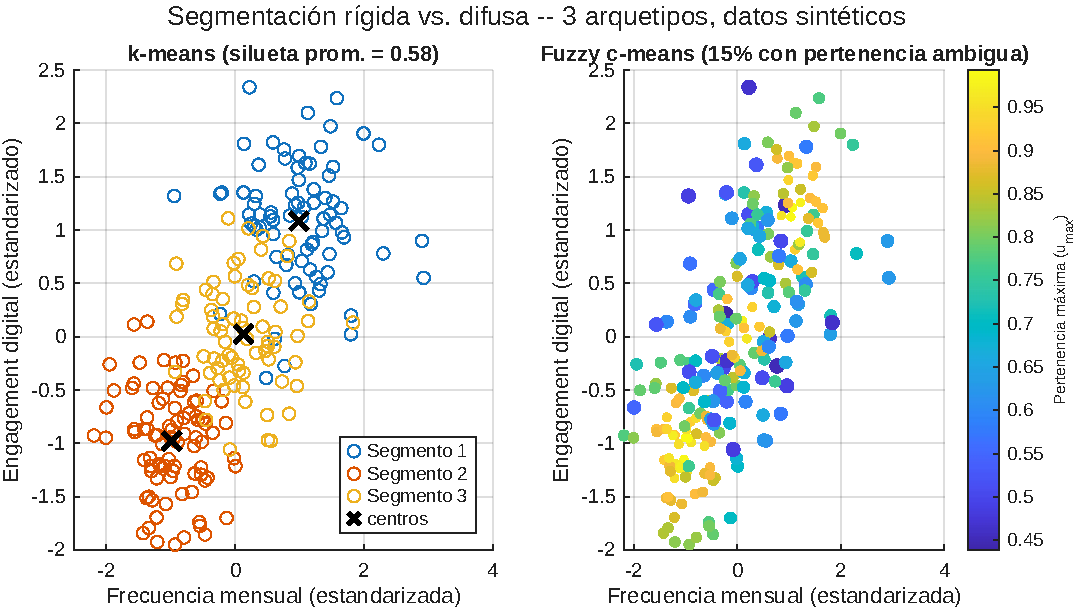
\includegraphics[width=0.98\textwidth]{figuras/matlab/cap02_segmentacion_comparacion.pdf}
  \captionof{figure}{Segmentación rígida (silueta promedio 0.58) vs. difusa
  (15\,\% de consumidores sin pertenencia dominante), con los tres arquetipos
  por defecto del script. Fuente: elaboración propia con datos sintéticos,
  \texttt{rng(42)}.}
  \label{fig:cap02-comparacion}
\end{center}

\begin{center}
  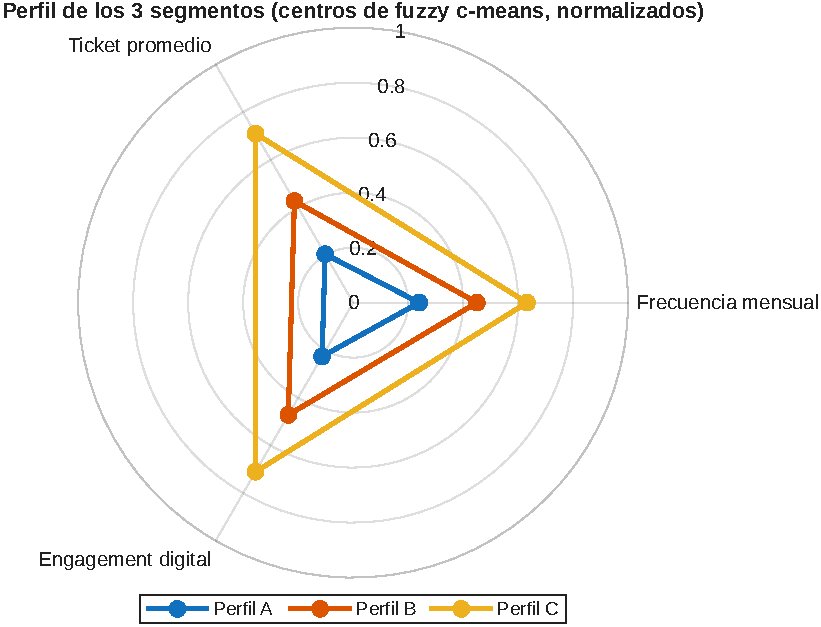
\includegraphics[width=0.62\textwidth]{figuras/matlab/cap02_perfiles_radar.pdf}
  \captionof{figure}{Perfil de los tres segmentos identificados por fuzzy
  c-means, centros normalizados, misma corrida. Fuente: elaboración propia
  con datos sintéticos.}
  \label{fig:cap02-radar}
\end{center}

\textbf{Interpretación de negocio.} El 15\,\% de los consumidores sintéticos
sin pertenencia dominante (figura~\ref{fig:cap02-comparacion}, panel
derecho, puntos de color intermedio y mayor tamaño) son, en términos de
negocio, los casos donde una campaña dirigida \enquote{solo al segmento leal} o
\enquote{solo al segmento ocasional} tiene la mayor probabilidad de desperdicio:
ese consumidor no es completamente ninguno de los dos, y tratarlo como si lo
fuera —en cualquiera de las dos direcciones— es un error de segmentación
sistemático, no aleatorio. El perfil C de la figura~\ref{fig:cap02-radar}
domina las tres variables simultáneamente: es el segmento \enquote{leal} de
alto valor, y su combinación de alta frecuencia, alto ticket y alto
engagement lo hace, en cualquier negocio real, el segmento prioritario de
retención.

\textbf{Ejercicio propuesto (usen exactamente este script, solo cambien el
bloque de parámetros).} Corran el script tres veces y completen un cuadro
con la silueta promedio y el \% de pertenencia ambigua de cada corrida:
\begin{enumerate}
  \item \textbf{Caso A — arquetipos por defecto:} los tres del script
  (\enquote{ocasional}, \enquote{leal}, \enquote{intermedio}).
  \item \textbf{Caso B — más traslape:} acerquen los tres centros entre sí
  (por ejemplo, reduzcan a la mitad la distancia entre las filas de
  \texttt{centrosTipicos}) sin cambiar las dispersiones.
  \item \textbf{Caso C — cuatro arquetipos:} agreguen una cuarta fila a
  \texttt{centrosTipicos} y a \texttt{dispersionTipica} con un arquetipo
  propio, y corran de nuevo.
\end{enumerate}
Con el cuadro completo, respondan por escrito: ¿qué le pasa a la silueta
promedio de k-means cuando los segmentos se acercan (Caso B)? ¿Qué le pasa
al \% de pertenencia ambigua? ¿Mejora o empeora la segmentación rígida al
añadir un cuarto segmento (Caso C)? Relacionen sus respuestas con el
criterio del codo (\textit{elbow method}) para elegir el número de
segmentos.

\textbf{Extensión opcional.} Sustituir los arquetipos sintéticos por datos
propios de un negocio digital al que el equipo tenga acceso legítimo
(exportación agregada y anonimizada de una tienda en línea propia, por
ejemplo) y repetir el análisis, documentando el consentimiento y anonimización
usados —enlace directo con el recuadro de Ética de este capítulo.
\end{cajaLaboratorio}

\begin{cajaEtica}
Construir un perfil de consumidor —rígido o difuso— a partir de datos de
comportamiento implica, por definición, vigilar y clasificar personas. El
laboratorio de este capítulo usa datos sintéticos precisamente para separar
el aprendizaje de la técnica de la pregunta ética de fondo: ¿bajo qué
condiciones es legítimo perfilar a un consumidor real? Como mínimo, el
perfilamiento con datos reales exige base legal para el tratamiento de
datos personales (retomado con detalle en el Cap. 3) y un propósito
declarado que el consumidor pueda conocer. Un modelo de segmentación
técnicamente impecable, construido sobre datos recolectados sin base legal,
no es un logro de análisis: es un incumplimiento con buena factura
estadística.
\end{cajaEtica}

\section{Estudio de caso}

\begin{casoFicticio}
Una cadena regional de gimnasios digitaliza su membresía y acumula, por
primera vez, datos de frecuencia de asistencia, uso de la app de
seguimiento y compra de productos adicionales (suplementos, ropa deportiva)
de sus 5{,}000 socios. El equipo de mercadotecnia propone segmentar con
k-means en cuatro perfiles fijos (\enquote{comprometido}, \enquote{ocasional},
\enquote{en riesgo de baja}, \enquote{nuevo}) para dirigir campañas de retención
distintas a cada uno. El equipo de datos advierte que, en una prueba
preliminar, casi una cuarta parte de los socios tiene un grado de
pertenencia similar a \enquote{comprometido} y a \enquote{en riesgo de baja} al
mismo tiempo.

\textbf{Preguntas guía.}
\begin{enumerate}
  \item ¿Qué error de mercadotecnia se comete si a ese 25\,\% \enquote{ambiguo}
  se le asigna, por la fuerza del algoritmo, a un solo segmento?
  \item Proponga una estrategia de comunicación específica para los socios
  con pertenencia dual \enquote{comprometido}/\enquote{en riesgo de baja}, distinta
  de la que recibiría cualquiera de los dos segmentos puros.
  \item ¿Qué variable adicional, no mencionada en el caso, ayudaría a
  distinguir mejor entre un socio genuinamente \enquote{en riesgo} y uno que
  solo tiene un patrón de asistencia irregular por temporada?
  \item Relacione este caso con la distinción de la sección~2.5 entre perfil
  como función del negocio y perfil como atributo fijo de la persona.
\end{enumerate}
\end{casoFicticio}

\section{Actividades y evidencias del portafolio}

\begin{description}
  \item[Reporte de indagación documental] Investigar y contrastar, con al
  menos dos fuentes, el uso de \textit{lookalike audiences} o públicos
  similares en una plataforma publicitaria real, y relacionarlo con el
  concepto de mercado meta digital (§2.2).
  \item[Exposición] Presentar, en equipo, uno de los ocho perfiles del Cubo
  NORISO \parencite{delgado2015noriso}, con un ejemplo ilustrado de consumo
  digital mexicano, dejando explícito que es una tipología de autor y no un
  hallazgo científico.
  \item[Solución de casos] Resolver el estudio de caso del gimnasio (§4) por
  escrito.
  \item[Reporte de debate] Debatir: ¿debería una organización pequeña, sin
  capacidad técnica para correr fuzzy c-means, renunciar a la segmentación
  difusa, o hay alternativas de menor costo para aproximarla?
  \item[Reporte de práctica] Entregar el cuadro de los tres casos del
  ejercicio propuesto del laboratorio (\S 3) —sin modificar el script, solo
  el bloque de parámetros— con las tres preguntas de comparación respondidas.
\end{description}

\section{Ruta de aprendizaje autónomo}

Dos horas de aprendizaje autónomo. Tareas concretas:
\begin{enumerate}
  \item Completar el Caso C del ejercicio propuesto (§3): agregar un cuarto
  arquetipo al bloque de parámetros de \texttt{cap02\_segmentacion.m} y
  registrar la silueta promedio resultante.
  \item Leer la ficha editorial de \textit{El Cubo NORISO}
  \parencite{delgado2015noriso} y resumir en un párrafo los ocho perfiles que
  propone.
  \item Revisar el Reporte de Resultados 9/25 de ENDUTIH 2024 y extraer un
  dato de radiografía del consumidor digital no incluido en el
  cuadro~\ref{tab:cap02-radiografia}.
\end{enumerate}

\section{Síntesis}

\begin{figure}[htbp]
  \centering
  % figuras/tikz/parte1-infografia-perfil.tex
% Infografía-modelo del perfil del consumidor digital (pieza de Parte I, §10).
% Sintetiza: variables de entrada -> método de construcción -> perfil resultante.
\begin{tikzpicture}[
    caja/.style={rectangle, rounded corners, draw=guindaIPN, thick, fill=guindaIPNClara,
                 minimum width=3.3cm, minimum height=1cm, align=center, font=\scriptsize},
    cajam/.style={rectangle, rounded corners, draw=bronceIPN, thick, fill=bronceIPNClaro,
                  minimum width=3.6cm, minimum height=1.9cm, align=center, font=\small},
    cajap/.style={rectangle, rounded corners, draw=guindaIPNOsc, thick, fill=white,
                  minimum width=3.3cm, minimum height=1.6cm, align=center, font=\small},
    flecha/.style={-{Stealth[length=3mm]}, thick, draw=doradoIPN}
  ]
  % Columna de variables (entrada)
  \node[caja] (geo) at (0,3) {Geográfica};
  \node[caja] (demo) at (0,1.7) {Demográfica};
  \node[caja] (psico) at (0,0.4) {Psicográfica};
  \node[caja] (cond) at (0,-0.9) {Conductual};

  % Método
  \node[cajam] (metodo) at (5,1.05) {\textbf{Método}\\ clustering rígido\\ ($k$-means) o difuso\\ (\textit{fuzzy c-means})};

  % Resultado
  \node[cajap] (perfil) at (10,1.05) {\textbf{Perfil}\\ función del\\ negocio que\\ lo construye};

  \foreach \n in {geo,demo,psico,cond} {
    \draw[flecha] (\n) -- (metodo);
  }
  \draw[flecha] (metodo) -- (perfil);

  \node[font=\scriptsize\itshape, text width=3.3cm, align=center] at (10,-0.4) {No es un atributo\\ fijo de la persona};
\end{tikzpicture}

  \caption{Infografía-modelo del perfil del consumidor digital: de las
  variables de entrada al perfil resultante, pasando por el método de
  construcción. Fuente: elaboración propia.}
  \label{fig:parte1-infografia-perfil}
\end{figure}

La segmentación digital no introdujo variables nuevas; abarató de forma
radical la variable conductual, antes la más cara de medir. El proceso STP
sigue vigente como marco de decisión, pero el método para llenarlo —cómo se
construyen los segmentos— tiene hoy una alternativa a la asignación rígida:
la pertenencia difusa, que reconoce lo que la segmentación tradicional
oculta por diseño, que una proporción no trivial de consumidores no encaja
por completo en ninguna casilla. No existe una tipología científica cerrada
de \enquote{tipos de perfil del consumidor digital}: existe un método —el
clustering, rígido o difuso— para construir tipologías propias a partir de
datos propios. Y el perfil resultante nunca es un atributo fijo de la
persona: es una función de qué negocio la está observando y qué variable de
éxito ese negocio optimiza.

\subsection*{Glosario del capítulo}
\begin{description}
  \item[Fuzzy c-means (FCM)] Algoritmo de segmentación que asigna a cada
  observación un grado de pertenencia parcial a cada segmento, en vez de una
  asignación única.
  \item[Grado de pertenencia ($u_{ik}$)] En FCM, valor entre 0 y 1 que
  cuantifica cuánto pertenece la observación $i$ al segmento $k$.
  \item[Mercado meta (\textit{target})] Segmento o segmentos hacia los que
  una organización dirige su oferta y comunicación.
  \item[Silueta (coeficiente de)] Medida de calidad de un agrupamiento
  rígido, que compara la cohesión interna de cada segmento contra su
  separación de los demás.
  \item[STP] Proceso de Segmentación, Targeting y Posicionamiento.
\end{description}

\subsection*{Autoevaluación}

\textbf{Opción múltiple}

\begin{enumerate}
  \item La fuente académica primaria de la segmentación de mercado es:
  \begin{enumerate}
    \item[a)] Kotler, P., \textit{Marketing Management}.
    \item[b)] Smith, W.R. (1956), \textit{Journal of Marketing}. \textit{(correcta)}
    \item[c)] Delgado Soriano et al. (2015), \textit{El Cubo NORISO}.
    \item[d)] Bezdek, J. (1981).
  \end{enumerate}
  \textit{Justificación:} §2.1.

  \item En fuzzy c-means, la segmentación rígida (k-means) corresponde al
  caso en que:
  \begin{enumerate}
    \item[a)] El número de segmentos es mayor a cuatro.
    \item[b)] Toda la pertenencia de cada observación se concentra en un solo segmento. \textit{(correcta)}
    \item[c)] No hay variables conductuales disponibles.
    \item[d)] El exponente difuso $m$ es igual a cero.
  \end{enumerate}
  \textit{Justificación:} recuadro de Frontera, §2.3.

  \item Según la radiografía del capítulo, la variable con mayor poder
  explicativo verificado del uso de internet en México es:
  \begin{enumerate}
    \item[a)] El nivel de estudios declarado.
    \item[b)] La edad, con caída sostenida a partir de los 35 años. \textit{(correcta)}
    \item[c)] El género.
    \item[d)] La marca de teléfono inteligente.
  \end{enumerate}
  \textit{Justificación:} §2.4, cuadro~\ref{tab:cap02-radiografia}.
\end{enumerate}

\textbf{Preguntas abiertas}

\begin{enumerate}
  \item Explique por qué el capítulo afirma que la segmentación rígida es un
  \enquote{caso límite} de la segmentación difusa, y no al revés.
  \textit{Clave:} la respuesta debe mostrar que fijar $u_{ik} \in \{0,1\}$
  con restricción de suma 1 es un caso particular de $u_{ik} \in [0,1]$ con
  la misma restricción; el conjunto de soluciones difusas incluye a las
  rígidas como subconjunto.
  \item ¿Por qué el capítulo sostiene que no existe un \enquote{perfil digital}
  único y portable de un consumidor entre industrias? \textit{Clave:} la
  respuesta debe apoyarse en que cada modelo de negocio mide una variable de
  éxito distinta (conversión, tiempo de permanencia, profundidad de
  producto), por lo que el perfil resultante depende de qué se mide, no es
  un atributo fijo de la persona (§2.5).
\end{enumerate}

\section{Lecturas recomendadas}

\begin{description}
  \item[\textcite{smith1956}] El artículo fundacional de la segmentación de
  mercado. Lectura obligada, breve, para entender el origen del STP antes de
  su sistematización posterior en manuales.
  \item[\textcite{delgado2015noriso}] Desarrolla el modelo del Cubo NORISO y
  sus ocho perfiles de personalidad del consumidor digital. Base recomendada
  para la exposición del portafolio de este capítulo.
  \item[\textcite{bezdek1981}] La formalización original del algoritmo fuzzy
  c-means. Técnica, densa; recomendada para el equipo que profundice en la
  extensión opcional del laboratorio.
\end{description}

% partes/parte1/cap03.tex
\chapter{Gestión de datos del consumidor: valor, omnicanalidad, escucha y decisión}
\label{cap:03}

\begin{cajaFicha}
\begin{description}
  \item[Unidad temática] I — Comportamiento, perfil y gestión de datos del consumidor digital.
  \item[Temas del programa] 1.3 Gestión de datos de los consumidores digitales: 1.3.1 Creación de valor para el consumidor-usuario (CX-UX); 1.3.2 Experiencias omnicanal consumidor-usuario (CX-UX); 1.3.3 Momentos de escucha a los consumidores digitales; 1.3.4 Importancia de la recolección y gestión de datos; 1.3.5 Toma de decisiones basadas en la gestión de datos digitales.
  \item[Horas] Teoría 2.0 · Práctica 5.0 · Aprendizaje autónomo 2.0.
  \item[Competencia de la unidad] Identifica el comportamiento del consumidor digital y su evolución a partir de sus tipos de perfil y gestión de datos.
  \item[Resultados de aprendizaje observables] Al concluir el capítulo, el estudiante:
  \begin{enumerate}
    \item distingue experiencia de cliente (CX) de experiencia de usuario (UX) y las ubica en el mapa de gestión de datos;
    \item aplica limpieza de datos, segmentación RFM y una prueba A/B para fundamentar una decisión;
    \item explica el marco legal mexicano vigente de protección de datos personales y sus implicaciones para la recolección de datos del consumidor.
  \end{enumerate}
  \item[Prerrequisitos] Cap. 1--2.
\end{description}
\end{cajaFicha}

\section{Caso de apertura}

Una cadena de farmacias mexicana descubre, al revisar sus datos de
fidelidad, que el 60\,\% de las personas que abandonan su carrito de compra
en la app lo hacen en el mismo paso: la solicitud de un segundo número
telefónico para verificación en dos pasos. Nadie diseñó ese paso para
espantar clientes. Se agregó por seguridad, se probó internamente, funcionó
bien. El dato de abandono —que solo existe porque la organización recolecta
y analiza sistemáticamente el comportamiento en su app— es lo que revela un
problema invisible al ojo humano. Este capítulo trata sobre esa cadena
completa: cómo se recolectan los datos, qué los vuelve confiables, cómo se
escucha al consumidor a través de ellos, y qué obligaciones legales trae
consigo tenerlos.

\section{Desarrollo teórico}

\begin{figure}[htbp]
  \centering
  \resizebox{\textwidth}{!}{% figuras/tikz/cap03-mapa-gestion-datos.tex
% Mapa de gestión de datos del consumidor digital: recolección -> decisión.
% Pieza de Parte I requerida por §10 del prompt de proyecto.
\begin{tikzpicture}[
    etapa/.style={rectangle, rounded corners, draw=guindaIPN, thick, fill=guindaIPNClara,
                  minimum width=2.5cm, minimum height=1.3cm, align=center, font=\scriptsize},
    flecha/.style={-{Stealth[length=2.8mm]}, thick, draw=doradoIPN}
  ]
  \node[etapa] (rec) at (0,0)    {Recolección\\ (§1.3.4)};
  \node[etapa] (lim) at (3,0)    {Limpieza y\\ calidad};
  \node[etapa] (esc) at (6,0)    {Escucha\\ (§1.3.3)};
  \node[etapa] (val) at (9,0)    {Creación\\ de valor\\ CX-UX (§1.3.1)};
  \node[etapa] (dec) at (12,0)   {Decisión\\ (§1.3.5)};

  \draw[flecha] (rec) -- (lim);
  \draw[flecha] (lim) -- (esc);
  \draw[flecha] (esc) -- (val);
  \draw[flecha] (val) -- (dec);

  \node[etapa, fill=terracotaIPNClara, draw=terracotaIPN, minimum width=11.5cm, minimum height=0.9cm]
    (base) at (5.5,-2) {Base legal y consentimiento (LFPDPPP) — condición de todo el mapa, no un paso más};
  \draw[flecha] (base.north -| rec) -- (rec.south);
  \draw[flecha] (base.north -| dec) -- (dec.south);
\end{tikzpicture}
}
  \caption{Mapa de gestión de datos del consumidor digital: de la
  recolección a la decisión, con la base legal como condición transversal, no
  como un paso más de la cadena. Fuente: elaboración propia.}
  \label{fig:cap03-mapa}
\end{figure}

\subsection{Creación de valor para el consumidor-usuario (CX-UX)}
\progtag{1.3.1}

CX (\textit{customer experience}, experiencia de cliente) y UX
(\textit{user experience}, experiencia de usuario) no son sinónimos, aunque
el capítulo del programa oficial las agrupe bajo una misma sigla compuesta y
buena parte de la bibliografía de comportamiento del consumidor las trate
como intercambiables \parencite{hoyer2024consumer}.
UX es el diseño de la interacción con un producto o interfaz específicos
—qué tan fácil es completar una tarea en una app—. CX es la suma de todas
las interacciones de una persona con una organización a lo largo del tiempo
y de los canales —de las cuales UX es una parte, no el todo—. Una app puede
tener una UX impecable (fácil de usar, rápida) dentro de una CX deficiente
(si, por ejemplo, el servicio al cliente detrás de esa app es lento o
inconsistente). Distinguir ambas evita el error común de optimizar la
interfaz mientras el resto de la relación con el cliente se deteriora sin
que ningún panel de control lo esté midiendo.

\subsection{Experiencias omnicanal consumidor-usuario (CX-UX)}
\progtag{1.3.2}

La definición académica de referencia es la de Verhoef, Kannan e Inman:
omnicanalidad es \enquote{la gestión sinérgica de los múltiples canales y
puntos de contacto disponibles, de forma que la experiencia del cliente a
través de los canales y el desempeño a través de los canales se optimicen}
\parencite{verhoef2015}. La palabra clave es \textit{sinérgica}: no basta con
que una organización esté presente en varios canales (multicanalidad); la
omnicanalidad exige que esos canales compartan una sola identidad de cliente
reconocible (figura~\ref{fig:cap03-omnicanal}), de modo que un consumidor que
empieza una compra en la app y la termina en tienda física sea tratado como
la misma persona, no como dos registros distintos.

\begin{figure}[htbp]
  \centering
  % figuras/tikz/cap03-omnicanal.tex
% Experiencias omnicanal: puntos de contacto distintos que deben resolver a
% una sola identidad de cliente (Verhoef, Kannan & Inman, 2015).
\begin{tikzpicture}[
    canal/.style={rectangle, rounded corners, draw=bronceIPN, thick, fill=bronceIPNClaro,
                  minimum width=2.4cm, minimum height=0.9cm, align=center, font=\scriptsize},
    centro/.style={circle, draw=guindaIPN, very thick, fill=guindaIPNClara,
                   minimum size=2.4cm, align=center, font=\small},
    flecha/.style={-{Stealth[length=2.5mm]}, thick, draw=doradoIPN}
  ]
  \node[centro] (id) at (0,0) {Identidad\\ única de\\ cliente};

  \node[canal] (app)    at (-4.2, 2.2) {App móvil};
  \node[canal] (web)    at (0, 3.2)    {Sitio web};
  \node[canal] (tienda) at (4.2, 2.2)  {Tienda física};
  \node[canal] (social) at (-4.2,-2.2) {Redes sociales};
  \node[canal] (cc)     at (4.2,-2.2)  {Centro de contacto};

  \foreach \n in {app,web,tienda,social,cc} {
    \draw[flecha] (\n) -- (id);
  }
\end{tikzpicture}

  \caption{Experiencia omnicanal: puntos de contacto distintos que deben
  resolver a una sola identidad de cliente. Fuente: elaboración propia con
  base en \parencite{verhoef2015}.}
  \label{fig:cap03-omnicanal}
\end{figure}

Resolver esa identidad única es, en la práctica, un problema técnico difícil
—el mismo problema que atraviesa el fin de las cookies de terceros y el giro
a datos de primera parte que se discute en el recuadro de Frontera de este
capítulo—, y también un problema legal: unificar el rastro de una persona
entre canales es, por definición, tratamiento de datos personales, sujeto a
la ley que se revisa en la §2.4.

\subsection{Momentos de escucha a los consumidores digitales}
\progtag{1.3.3}

\enquote{Escuchar} a un consumidor digital no significa, la mayor parte del
tiempo, leer lo que escribe. Significa observar tres tipos de señal
distintos: la señal declarada (lo que el consumidor dice explícitamente —una
reseña, una encuesta, un comentario en redes—), la señal conductual (lo que
el consumidor hace —qué compra, dónde se detiene, qué abandona—) y la señal
de contexto (las circunstancias en que ocurre la interacción —hora, canal,
dispositivo—). El caso de apertura de este capítulo es un ejemplo de escucha
puramente conductual: nadie tuvo que quejarse del segundo número telefónico
para que el problema fuera visible en los datos. Un programa de escucha que
solo atiende la señal declarada (encuestas de satisfacción, menciones en
redes) sistemáticamente subestima estos problemas silenciosos, porque la
mayoría de los consumidores que abandonan una compra no se queja: simplemente
se va.

\subsection{Importancia de la recolección y gestión de datos}
\progtag{1.3.4}

\begin{cajaFrontera}
\textbf{Datos de primera y de cero parte, y el mito del fin de las cookies de
terceros.} \enquote{Datos de primera parte} son los que una organización
recolecta directamente de su propia relación con el consumidor (compras,
registro, navegación en su propio sitio); \enquote{datos de cero parte} son los
que el consumidor entrega de forma voluntaria y explícita (una encuesta de
preferencias, un cuestionario de talla). Ambos ganaron relevancia
estratégica por presión regulatoria (la LFPDPPP que se revisa en la §2.4) y
por el supuesto fin de las cookies de terceros en los navegadores. Pero ese
supuesto fin no ocurrió como se anunció: Google revirtió en 2024 su plan de
depreciación de cookies de terceros en Chrome, descartó también el mecanismo
alternativo de \textit{choice prompt} en abril de 2025, y retiró las APIs de
reemplazo de Privacy Sandbox en octubre de 2025
\parencite{eprs2025darkpatterns}. \textbf{Vigente a septiembre de 2026:} las
cookies de terceros siguen activas por defecto en Chrome. El giro hacia
datos de primera y de cero parte sigue siendo la estrategia correcta —por
razones de confianza del consumidor y de cumplimiento legal, no solo
técnicas—, pero el capítulo advierte contra repetir la narrativa de
\enquote{las cookies ya desaparecieron}, que circula ampliamente en el
discurso de mercadotecnia digital sin corresponder a los hechos verificables
a la fecha de este libro.
\end{cajaFrontera}

El marco legal mexicano de protección de datos personales cambió de forma
sustancial en 2025. El cuadro~\ref{tab:cap03-lfpdppp} resume la cronología
verificada contra fuentes oficiales.

\begin{table}[htbp]
\centering
\begin{tabular}{@{}p{2.6cm}p{9.6cm}@{}}
\toprule
Fecha & Hecho jurídico \\
\midrule
20-dic-2024 & Reforma constitucional de simplificación orgánica: se decreta la desaparición del INAI, entre otros seis organismos autónomos \parencite{dof_simplificacion2024}. \\
20-mar-2025 & Se publica en el DOF la nueva Ley Federal de Protección de Datos Personales en Posesión de los Particulares (LFPDPPP), que abroga la ley de 2010; entra en vigor al día siguiente \parencite{dof_lfpdppp2025}. \\
9-may-2025 & Se formaliza la entrega-recepción institucional del INAI a la Secretaría Anticorrupción y Buen Gobierno, que asume las atribuciones de protección de datos personales de particulares \parencite{sabg2025entregarecepcion}. \\
14-nov-2025 & Reforma de homologación normativa a la LFPDPPP \parencite{dof_lfpdppp_reforma2025nov}. \\
\bottomrule
\end{tabular}
\caption{Cronología verificada de la reforma a la protección de datos
personales en México. Fuente: elaboración propia con base en el Diario
Oficial de la Federación y comunicados oficiales de gob.mx.}
\label{tab:cap03-lfpdppp}
\end{table}

Hay un punto de la nueva ley que este libro presenta con cautela deliberada,
en vez de con una postura firme: según fuentes de análisis jurídico
corporativo consultadas en la investigación de este libro, la nueva LFPDPPP
establecería el consentimiento tácito como regla general para el tratamiento
de datos personales —salvo datos sensibles—, mientras que, según esas mismas
fuentes, la ley también exigiría que el consentimiento sea libre, específico
e informado. Esta aparente tensión entre ambos principios no se resuelve en
este libro: se señala explícitamente para que el estudiante sepa que existe,
y se recomienda consultar el texto vigente de la ley y, para una decisión
profesional real, a un especialista en derecho de protección de datos antes
de diseñar un mecanismo de consentimiento con implicaciones legales.

\subsection{Toma de decisiones basadas en gestión de datos digitales}
\progtag{1.3.5}

La mercadotecnia impulsada por datos (\textit{data-driven marketing}) es uno
de los ejes centrales de la lectura contemporánea del marketing digital
\parencite{kotler2021marketing50}. Un dato limpio, bien recolectado y con
base legal es una condición necesaria para decidir bien; no es, por sí sola,
condición suficiente. Hace
falta, además, un método que traduzca el dato en decisión sin engañarse a
sí mismo por diseño. El laboratorio de este capítulo desarrolla tres de esos
métodos, en orden creciente de exigencia: limpiar datos antes de usarlos,
segmentar clientes por valor con RFM, y —el más exigente de los tres— probar
una decisión con un experimento controlado (A/B) en vez de decidir por
intuición o por la primera diferencia que se observe en un panel.

\section{Evidencia de México y del mundo}

\begin{table}[htbp]
\centering
\begin{tabular}{@{}lr@{}}
\toprule
Indicador (2024) & Cifra \\
\midrule
Personas con al menos un producto financiero formal & 76.5\,\% \\
Brecha de género en tenencia de producto financiero & 72.8\,\% mujeres vs. 80.9\,\% hombres \\
Personas que llevan registro de sus gastos o los de su hogar & 65.3\,\% \\
\bottomrule
\end{tabular}
\caption{Indicadores de gestión de información financiera personal en
México. Fuente: elaboración propia con datos de INEGI/CNBV, Encuesta
Nacional de Inclusión Financiera (ENIF) 2024, Comunicado de prensa 49/25
\parencite{inegi2025enif}.}
\label{tab:cap03-enif}
\end{table}

El dato de la brecha de género en el cuadro~\ref{tab:cap03-enif} —ocho
puntos porcentuales— es relevante para este capítulo más allá de su interés
demográfico: cualquier organización que segmente por comportamiento
financiero sin ponderar esta brecha corre el riesgo de que su definición de
\enquote{cliente de alto valor} termine, sin proponérselo, subrepresentando a
las mujeres del mercado que analiza —un ejemplo concreto de cómo una decisión
técnica de segmentación (§2 del Cap. 2) puede heredar un sesgo social ya
presente en los datos de origen, sin que ningún paso del proceso lo haga
explícito. La brecha se enmarca, además, en un crecimiento general de la
conectividad mexicana —86.1\,\% de la población de 6 años o más ya usa
internet en 2025 \parencite{inegi2026endutih}— que hace cada vez más costoso,
en términos de mercado potencial no capturado, ignorar sesgos de este tipo
en el diseño de un sistema de gestión de datos.

\section{Laboratorio MATLAB: RFM, CLV y prueba A/B}

\begin{cajaLaboratorio}
\textbf{Objetivo.} Limpiar un conjunto de datos transaccionales con valores
faltantes y atípicos, segmentar clientes por valor con el método RFM
(Recencia, Frecuencia, Monto), calcular un valor de vida del cliente (CLV)
simple, y decidir entre dos versiones de una página de checkout con una
prueba A/B basada en un test estadístico, no en la simple comparación de
porcentajes.

\textbf{Concepto detrás del código.} RFM puntúa a cada cliente en tres
dimensiones (recencia: qué tan reciente fue su última compra; frecuencia:
cuántas compras hizo; monto: cuánto gastó en promedio), típicamente por
quintiles, y combina los tres puntajes en un segmento. El CLV simple usado
aquí es
\[
  \mathrm{CLV}_i = \text{monto}_i \times \text{frecuencia}_i \times \text{horizonte (años)},
\]
una aproximación didáctica —no incorpora tasa de descuento ni probabilidad
de retención, que un CLV de negocio real sí debería considerar—. La prueba
A/B compara dos proporciones (tasa de conversión de la versión A vs. B) con
un test $z$ de dos proporciones:
\[
  z = \frac{\hat{p}_B - \hat{p}_A}{\sqrt{\hat{p}(1-\hat{p})\left(\frac{1}{n_A}+\frac{1}{n_B}\right)}},
  \qquad \hat{p} = \frac{x_A + x_B}{n_A + n_B},
\]
donde $\hat{p}$ es la proporción conjunta bajo la hipótesis nula de que
ambas versiones convierten igual.

\textbf{Script.} \texttt{matlab/cap03/cap03\_rfm\_clv\_ab.m}. Es el
\textbf{mismo script, sin modificar}, que se usa en la Práctica 2 de esta
Parte. Corrida tal como está, usa 300 clientes \textbf{sintéticos}
(\texttt{rng(42)}), con 5\,\% de valores faltantes y 2\,\% de atípicos
introducidos a propósito para que el bloque de limpieza tenga un problema
real que resolver.

\begin{lstlisting}[style=MATLABStyle, caption={Bloque de parámetros editable (\texttt{cap03\_rfm\_clv\_ab.m}) — es lo único que cambia entre corridas.}]
nClientes = 300;    % tamano de la base sintetica (Bloques 1-2)
horizonteAnios = 3; % horizonte del CLV simple
alfa = 0.05;         % significancia de la prueba A/B (Bloque 3)
nA = 1200; conversionesA = 132;   % version A (control)
nB = 1180; conversionesB = 159;   % version B (variante)
\end{lstlisting}

\textbf{Salida esperada.} Dos figuras: distribución de segmentos RFM y CLV
promedio por segmento (figura~\ref{fig:cap03-rfmclv}), y resultado de la
prueba A/B con intervalos de confianza (figura~\ref{fig:cap03-ab}).

\begin{center}
  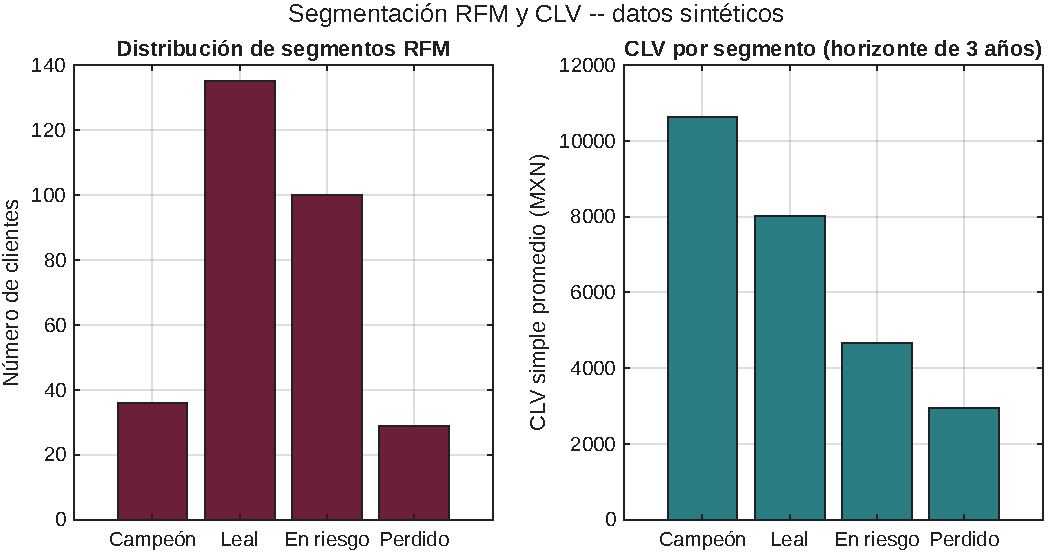
\includegraphics[width=0.98\textwidth]{figuras/matlab/cap03_rfm_clv.pdf}
  \captionof{figure}{Segmentación RFM (izquierda) y CLV simple promedio por
  segmento (derecha). Fuente: elaboración propia con datos sintéticos,
  \texttt{rng(42)}.}
  \label{fig:cap03-rfmclv}
\end{center}

\begin{center}
  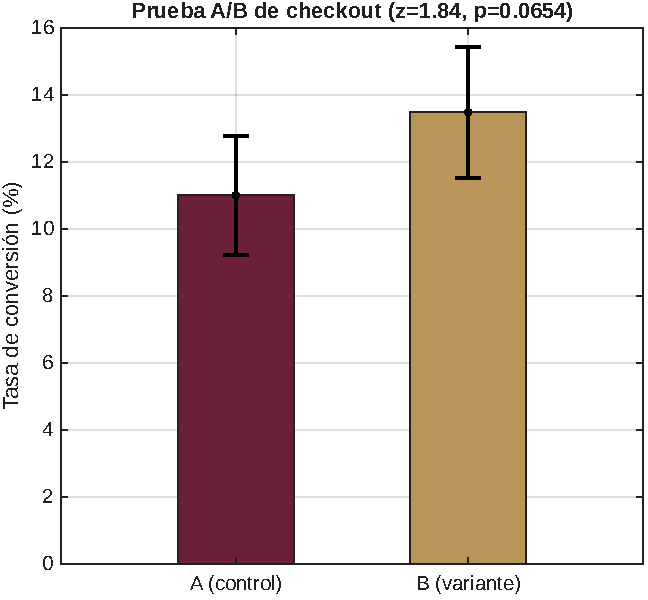
\includegraphics[width=0.62\textwidth]{figuras/matlab/cap03_prueba_ab.pdf}
  \captionof{figure}{Prueba A/B de checkout: la versión B convierte 2.5
  puntos porcentuales más, pero la diferencia no alcanza significancia
  estadística al 95\,\% ($p=0.065$). Fuente: elaboración propia con datos
  sintéticos.}
  \label{fig:cap03-ab}
\end{center}

\textbf{Interpretación de negocio.} El resultado de la prueba A/B es
deliberadamente el más instructivo del laboratorio: la versión B parece
mejor a simple vista (13.5\,\% contra 11.0\,\% de conversión), y un equipo
que decida \enquote{por el ojo} adoptaría B sin dudar —exactamente el tipo de
juicio bajo incertidumbre que Tversky y Kahneman documentan como propenso a
la heurística de representatividad, ver diferencia donde solo hay ruido
muestral \parencite{tverskykahneman1974}. El test estadístico
dice otra cosa: con $p=0.065$, apenas por encima del umbral convencional de
0.05, la diferencia observada es compatible con el azar. Los intervalos de
confianza de la figura~\ref{fig:cap03-ab} se traslapan de forma visible, lo
que confirma la misma conclusión sin necesidad de leer el valor $p$. La
decisión correcta no es \enquote{B es mejor, cámbiate} ni \enquote{no hay
diferencia, no importa}: es reconocer que la muestra actual no permite
concluir con la confianza convencional, y que la opción disciplinada es
correr la prueba más tiempo o con más tráfico antes de decidir —exactamente
el tipo de paciencia que la presión de negocio, en la práctica, más cuesta
sostener.

\textbf{Ejercicio propuesto (usen exactamente este script, solo cambien el
bloque de parámetros).} Corran el script tres veces y completen un cuadro
con la conversión de cada versión, el estadístico $z$, el valor $p$ y la
decisión que imprime cada corrida:
\begin{enumerate}
  \item \textbf{Caso A — valores por defecto:} $n_A=1200$, conversiones$_A=132$;
  $n_B=1180$, conversiones$_B=159$; $\alpha=0.05$.
  \item \textbf{Caso B — mismas tasas, más muestra:} multipliquen por 5 los
  cuatro valores de la prueba A/B ($n_A=6000$, conversiones$_A=660$;
  $n_B=5900$, conversiones$_B=795$), sin cambiar $\alpha$.
  \item \textbf{Caso C — mismos datos del Caso A, umbral más laxo:}
  regresen a los valores del Caso A y cambien solo $\alpha$ a 0.10.
\end{enumerate}
Con el cuadro completo, respondan por escrito: ¿cambia la decisión entre el
Caso A y el Caso B, aunque las proporciones observadas sean idénticas? ¿A
qué se debe? ¿Cambia la decisión entre el Caso A y el Caso C? ¿Qué tipo de
error (falso positivo o falso negativo) se vuelve más probable al relajar
$\alpha$, y en qué escenarios de negocio sería aceptable correr ese riesgo?

\textbf{Extensión opcional.} Incorporar una tasa de descuento al cálculo de
CLV (CLV descontado a valor presente) y comparar el orden resultante de los
cuatro segmentos contra el CLV simple del script.
\end{cajaLaboratorio}

\begin{cajaEtica}
La reforma a la LFPDPPP resumida en el cuadro~\ref{tab:cap03-lfpdppp} sigue
activa: hubo una reforma en noviembre de 2025 y es razonable esperar más
ajustes. Ninguna decisión de recolección de datos de este capítulo —ni la
resolución de identidad omnicanal, ni la segmentación RFM con datos reales,
ni ningún mecanismo de consentimiento— debe diseñarse a partir de lo que
diga este libro como fuente única. La responsabilidad profesional incluye
verificar el estado vigente de la ley al momento de implementar, no solo al
momento de estudiar.
\end{cajaEtica}

\section{Estudio de caso}

\begin{casoFicticio}
Una plataforma de cursos en línea nota que su tasa de finalización de
cursos gratuitos es del 8\,\%, y decide probar un rediseño del panel de
progreso del estudiante (barra de avance más visible, recordatorios por
correo). Corre una prueba A/B durante dos semanas con 400 estudiantes por
grupo: la versión con el rediseño muestra una finalización de 11\,\%, contra
8.5\,\% de la versión de control. El equipo de producto presenta el
resultado a la dirección como \enquote{el rediseño aumenta la finalización 3
puntos porcentuales, hay que lanzarlo a todos los usuarios}.

\textbf{Preguntas guía.}
\begin{enumerate}
  \item Con los datos dados (400 y 400 estudiantes, 11\,\% y 8.5\,\%),
  replique el cálculo del test $z$ de dos proporciones del laboratorio y
  determine si la diferencia es estadísticamente significativa al 95\,\%.
  \item Si el resultado no fuera significativo, ¿qué le respondería al
  equipo de producto que quiere lanzar el cambio de inmediato?
  \item ¿Qué otros datos —más allá de la tasa de finalización— ayudarían a
  decidir si vale la pena el costo de desarrollo del rediseño, incluso si la
  diferencia fuera significativa?
  \item Relacione este caso con la distinción entre señal declarada y señal
  conductual de la §2.3: ¿en qué categoría cae la tasa de finalización de
  cursos?
\end{enumerate}
\end{casoFicticio}

\section{Actividades y evidencias del portafolio}

\begin{description}
  \item[Reporte de indagación documental] Consultar el texto vigente de la
  LFPDPPP en el sitio de la Secretaría Anticorrupción y Buen Gobierno y
  resumir, con cita textual de máximo 40 palabras, el artículo que regula el
  consentimiento para el tratamiento de datos personales.
  \item[Exposición] Presentar la diferencia entre CX y UX con un ejemplo real
  de una organización mexicana (app, sitio o servicio digital) donde una de
  las dos esté claramente mejor atendida que la otra.
  \item[Solución de casos] Resolver el estudio de caso de la plataforma de
  cursos en línea (§4) con el cálculo estadístico completo.
  \item[Reporte de prácticas] Documentar, paso por paso, la ejecución del
  laboratorio MATLAB de este capítulo (bloques 1--3), con capturas de las
  dos figuras y una interpretación propia de al menos un párrafo por bloque.
\end{description}

\section{Ruta de aprendizaje autónomo}

Dos horas de aprendizaje autónomo. Tareas concretas:
\begin{enumerate}
  \item Completar el Caso B del ejercicio propuesto (§5, multiplicar por 5
  la muestra de la prueba A/B) y registrar si la decisión cambia respecto al
  Caso A.
  \item Investigar si, a la fecha en que se realice esta tarea, hay una
  reforma o disposición nueva a la LFPDPPP posterior a noviembre de 2025, y
  documentarla con fuente oficial.
  \item Calcular a mano el CLV simple de un cliente hipotético propio
  (monto, frecuencia y horizonte definidos por el estudiante) y verificar el
  resultado con el script del laboratorio.
\end{enumerate}

\section{Síntesis}

La gestión de datos del consumidor digital es una cadena, no un evento
aislado: recolección, limpieza, escucha, creación de valor y decisión, con
la base legal como condición transversal de toda la cadena, no como un
trámite al final. CX y UX son conceptos distintos que conviene no fusionar.
La omnicanalidad exige resolver una identidad única de cliente entre
canales, tarea que es a la vez técnica y legal. El marco mexicano de
protección de datos personales cambió de fondo en 2025, con una tensión
normativa —consentimiento tácito frente a consentimiento informado— que este
libro no resuelve por sí solo. Y ninguna decisión basada en datos es mejor
que el rigor del método que la sostiene: la comparación simple de
porcentajes en una prueba A/B, sin prueba estadística, es la forma más común
de auto-engaño con buena presentación visual.

\subsection*{Glosario del capítulo}
\begin{description}
  \item[CLV (\textit{customer lifetime value})] Valor de vida del cliente:
  ingreso esperado que un cliente generará a lo largo de su relación con la
  organización.
  \item[CX (\textit{customer experience})] Suma de todas las interacciones de
  una persona con una organización a lo largo del tiempo y los canales.
  \item[Datos de cero parte] Datos que el consumidor entrega de forma
  voluntaria y explícita.
  \item[Datos de primera parte] Datos que una organización recolecta
  directamente de su propia relación con el consumidor.
  \item[Nivel de significancia ($\alpha$)] Umbral de probabilidad, definido
  antes de la prueba, por debajo del cual se considera que una diferencia
  observada es \enquote{estadísticamente significativa}. Rango: $\alpha \in
  (0,1)$; valores convencionales en la práctica son 0.01, 0.05 y 0.10 (el
  script de este capítulo usa 0.05 por defecto, editable).
  \item[Omnicanalidad] Gestión sinérgica de múltiples canales de forma que la
  experiencia y el desempeño del cliente se optimicen a través de ellos.
  \item[Puntaje RFM] Suma de los tres puntajes por quintil (recencia,
  frecuencia, monto), cada uno en el rango entero 1--5. Rango del puntaje
  total: 3 (el peor caso posible) a 15 (el mejor).
  \item[RFM] Método de segmentación por Recencia, Frecuencia y Monto de
  compra.
  \item[UX (\textit{user experience})] Diseño de la interacción con un
  producto o interfaz específicos.
  \item[Valor $p$] Probabilidad de observar una diferencia al menos tan
  grande como la registrada si, en realidad, no hubiera diferencia entre las
  dos versiones (hipótesis nula). Rango: $p \in [0,1]$; se rechaza la
  hipótesis nula cuando $p < \alpha$.
\end{description}

\subsection*{Autoevaluación}

\textbf{Opción múltiple}

\begin{enumerate}
  \item La diferencia central entre CX y UX es que:
  \begin{enumerate}
    \item[a)] Son sinónimos intercambiables.
    \item[b)] UX es el diseño de una interacción específica; CX es la suma de todas las interacciones a través del tiempo y los canales. \textit{(correcta)}
    \item[c)] CX aplica solo a apps móviles.
    \item[d)] UX es responsabilidad legal; CX es responsabilidad de diseño.
  \end{enumerate}
  \textit{Justificación:} §2.1.

  \item Según la cronología verificada en este capítulo, la nueva LFPDPPP
  entró en vigor:
  \begin{enumerate}
    \item[a)] El 20 de diciembre de 2024.
    \item[b)] El 21 de marzo de 2025. \textit{(correcta)}
    \item[c)] El 9 de mayo de 2025.
    \item[d)] El 14 de noviembre de 2025.
  \end{enumerate}
  \textit{Justificación:} cuadro~\ref{tab:cap03-lfpdppp}.

  \item En la prueba A/B del laboratorio, un valor $p=0.065$ con
  $\alpha=0.05$ significa que:
  \begin{enumerate}
    \item[a)] La versión B es definitivamente mejor.
    \item[b)] No hay evidencia suficiente para rechazar la hipótesis de que ambas versiones convierten igual. \textit{(correcta)}
    \item[c)] El experimento falló y debe descartarse.
    \item[d)] La versión A es mejor.
  \end{enumerate}
  \textit{Justificación:} §5, interpretación de negocio.
\end{enumerate}

\textbf{Preguntas abiertas}

\begin{enumerate}
  \item Explique, con el caso de apertura del capítulo, la diferencia entre
  escucha declarada y escucha conductual. \textit{Clave:} la respuesta debe
  señalar que el problema del segundo número telefónico se detectó sin que
  ningún cliente se quejara explícitamente —es decir, por señal conductual
  (abandono en un paso específico), no por señal declarada.
  \item ¿Por qué el capítulo presenta la tensión entre consentimiento tácito
  y consentimiento informado en la LFPDPPP sin resolverla?
  \textit{Clave:} la respuesta debe reconocer que es una aparente
  contradicción encontrada en fuentes de análisis jurídico, no confirmada
  contra el texto legal completo, y que resolverla con una postura firme sin
  esa verificación sería una afirmación legal no sustentada.
\end{enumerate}

\section{Lecturas recomendadas}

\begin{description}
  \item[\textcite{verhoef2015}] El artículo fundacional de la omnicanalidad,
  con la definición que usa este capítulo. Introducción breve a un número
  especial de \textit{Journal of Retailing}.
  \item[\textcite{dof_lfpdppp2025}] El texto oficial de la nueva LFPDPPP.
  Lectura obligada para cualquier reporte de indagación documental de este
  capítulo que involucre datos personales.
  \item[\textcite{mathur2019}] Aunque se desarrolla con detalle en el Cap. 7,
  esta taxonomía empírica de patrones oscuros en 11{,}000 sitios de comercio
  electrónico es una lectura útil para entender los límites éticos de la
  \enquote{toma de decisiones basada en datos} de la §2.5.
\end{description}

% partes/parte1/cap04.tex
\chapter{Base tecnológica: buscadores, plataformas, redes y comercio electrónico}
\label{cap:04}

\begin{cajaFicha}
\begin{description}
  \item[Unidad temática] I — Comportamiento, perfil y gestión de datos del consumidor digital.
  \item[Temas del programa] 1.4 Base tecnológica para la gestión de datos de los consumidores digitales: 1.4.1 Temas selectos de buscadores y plataformas de gestión integral, redes sociales y comercio electrónico.
  \item[Horas] Teoría 2.0 · Práctica 3.0 · Aprendizaje autónomo 1.0.
  \item[Competencia de la unidad] Identifica el comportamiento del consumidor digital y su evolución a partir de sus tipos de perfil y gestión de datos.
  \item[Resultados de aprendizaje observables] Al concluir el capítulo, el estudiante:
  \begin{enumerate}
    \item aplica una matriz de criterios durables para evaluar cualquier plataforma digital, presente o futura;
    \item interpreta una serie de interés de búsqueda en sus componentes de tendencia y estacionalidad;
    \item extrae y analiza frecuencia de términos de un corpus de escucha social.
  \end{enumerate}
  \item[Prerrequisitos] Cap. 1--3.
\end{description}
\end{cajaFicha}

\section{Caso de apertura}

\textbf{Vigente a septiembre de 2026.} En 2020, buena parte del material de
mercadotecnia digital advertía que las cookies de terceros desaparecerían de
Chrome en un plazo de dos o tres años. No ocurrió (Cap.~3, §2.4). En 2024,
Gartner predijo que el volumen de búsqueda tradicional caería 25\,\% para
2026 por efecto de los chatbots de IA. Al cierre de este libro, las propias
fuentes de industria se contradicen sobre si esa caída ocurrió tal cual se
predijo. Este capítulo parte de una premisa incómoda pero honesta: cualquier
cifra puntual de cuota de mercado o de adopción tecnológica que aparezca
aquí puede estar desactualizada antes de que el estudiante egrese. Por eso
el capítulo no enseña un catálogo de plataformas —enseña los criterios para
evaluar cualquier plataforma, presente o futura, sin depender de que ninguna
marca en particular siga existiendo.

\section{Desarrollo teórico}

\subsection{Temas selectos de buscadores y plataformas: una matriz de criterios durables}
\progtag{1.4.1}

El programa oficial deja este subtema deliberadamente abierto
—\enquote{temas selectos}— precisamente porque el panorama tecnológico cambia
más rápido que cualquier edición impresa de un libro de texto. La respuesta
de este capítulo no es listar herramientas vigentes hoy (que envejecerán),
sino ofrecer cuatro criterios de análisis que se sostienen con independencia
de qué marca domine el mercado en el momento en que se lean
(figura~\ref{fig:cap04-criterios}).

\begin{figure}[htbp]
  \centering
  % figuras/tikz/cap04-criterios-evaluacion.tex
% Matriz de criterios de evaluación de plataformas digitales, diseñada para
% sobrevivir al cambio de marcas concretas (§5.7 del prompt de proyecto).
\begin{tikzpicture}[
    criterio/.style={rectangle, rounded corners, draw=guindaIPN, thick, fill=guindaIPNClara,
                     minimum width=5.6cm, minimum height=1.15cm, align=left, font=\scriptsize},
  ]
  \node[criterio] (c1) at (0,3.3)  {\textbf{Modelo de negocio}\\ publicidad / suscripción / comisión transaccional};
  \node[criterio] (c2) at (0,1.9)  {\textbf{Intermediación de datos}\\ ¿quién controla el dato del consumidor?};
  \node[criterio] (c3) at (0,0.5)  {\textbf{Interoperabilidad}\\ APIs abiertas vs. cerradas};
  \node[criterio] (c4) at (0,-0.9) {\textbf{Exposición regulatoria}\\ DSA europea, LFPDPPP mexicana};

  \node[font=\small\bfseries, align=center, text width=3.2cm] at (5.2,1.2)
    {Evaluar cualquier\\ plataforma o\\ herramienta\\ vigente con estos\\ cuatro criterios};
  \draw[-{Stealth[length=3mm]}, thick, draw=doradoIPN] (3.0,1.2) -- (3.9,1.2);
\end{tikzpicture}

  \caption{Matriz de criterios durables para evaluar buscadores, plataformas
  y redes sociales, con independencia de la marca vigente. Fuente:
  elaboración propia.}
  \label{fig:cap04-criterios}
\end{figure}

El cuadro~\ref{tab:cap04-criterios} desarrolla cada criterio con la pregunta
concreta que un mercadólogo digital debería hacerse frente a cualquier
plataforma —la que use hoy, o la que la reemplace mañana—.

\begin{table}[htbp]
\centering
\begin{tabular}{@{}p{3.3cm}p{9.1cm}@{}}
\toprule
Criterio & Pregunta de evaluación \\
\midrule
Modelo de negocio & ¿La plataforma se financia por publicidad, suscripción o comisión transaccional? Cada modelo alinea sus incentivos de forma distinta con los intereses del consumidor. \\
Intermediación de datos & ¿Quién es dueño del dato de comportamiento del consumidor generado en la plataforma: la organización que anuncia, la plataforma, o ambas bajo condiciones específicas? \\
Interoperabilidad & ¿La plataforma ofrece APIs abiertas que permiten exportar datos propios, o mantiene los datos cautivos dentro de su ecosistema cerrado? \\
Exposición regulatoria & ¿Qué marco normativo aplica a la plataforma (DSA europea, LFPDPPP mexicana, ninguno vigente todavía) y qué riesgo de cumplimiento implica usarla? \\
\bottomrule
\end{tabular}
\caption{Matriz de criterios durables para evaluar plataformas digitales.
Fuente: elaboración propia, síntesis del criterio metodológico desarrollado
en la investigación de este capítulo.}
\label{tab:cap04-criterios}
\end{table}

\begin{cajaFrontera}
\textbf{El comercio agéntico como nueva capa de intermediación.} Esta capa
es una de las tendencias que \textit{Marketing 6.0} anticipa bajo la
etiqueta de tecnología inmersiva aplicada al consumo
\parencite{kotler2024marketing6} (Cap.~1, §2.1). A
septiembre de 2026, el llamado \enquote{comercio agéntico} —asistentes de
compra basados en modelos de lenguaje que buscan, comparan y en ocasiones
ejecutan la transacción en nombre del consumidor— opera a escala, con al
menos dos protocolos abiertos en competencia (el Agentic Commerce Protocol
de Stripe y OpenAI, y el Universal Commerce Protocol de Google, presentado
en NRF 2026) y el enfoque propietario de Amazon (Rufus, Alexa+), que no se
ha sumado a ningún protocolo abierto. Aplicando la matriz de este capítulo:
el criterio más relevante no es qué asistente tiene más usuarios este
trimestre —cifra que cambiará antes de la próxima edición del libro—, sino
quién controla la capa de intermediación entre el consumidor y el punto de
venta (figura~\ref{fig:cap04-agentico}). Esa pregunta estructural sí
sobrevive al cambio de marcas —y no es retórica: la taxonomía empírica de
patrones oscuros de Mathur et al. \parencite{mathur2019} muestra que
cualquier capa de intermediación con suficiente control sobre la interfaz
puede, sin cambiar de tecnología, pasar de facilitar la decisión del
consumidor a sesgarla.
\end{cajaFrontera}

\begin{figure}[htbp]
  \centering
  % figuras/tikz/cap04-comercio-agentico.tex
% El comercio agéntico como nueva capa de intermediación entre el
% consumidor y el comercio electrónico (vigente a septiembre de 2026).
\begin{tikzpicture}[
    nodo/.style={rectangle, rounded corners, draw=guindaIPN, thick, fill=guindaIPNClara,
                 minimum width=3cm, minimum height=1.1cm, align=center, font=\small},
    nodom/.style={rectangle, rounded corners, draw=doradoIPN, very thick, fill=bronceIPNClaro,
                  minimum width=4.2cm, minimum height=1.3cm, align=center, font=\small},
    flecha/.style={-{Stealth[length=3mm]}, thick, draw=grisIPN}
  ]
  \node[nodo] (consumidor) at (0,0) {Consumidor};
  \node[nodom] (agente) at (5,0) {\textbf{Agente de IA}\\ (protocolo ACP / UCP)};
  \node[nodo] (comercio) at (10,0) {Comercio\\ electrónico};

  \draw[flecha] (consumidor) -- node[above, font=\scriptsize] {intención de compra} (agente);
  \draw[flecha] (agente) -- node[above, font=\scriptsize, align=center] {búsqueda, comparación,\\ transacción} (comercio);

  \node[font=\scriptsize\itshape, text width=4.2cm, align=center] at (5,-1.4)
    {Pregunta estructural: ¿quién controla esta capa de intermediación?};
\end{tikzpicture}

  \caption{El comercio agéntico como capa de intermediación entre el
  consumidor y el comercio electrónico. Fuente: elaboración propia.}
  \label{fig:cap04-agentico}
\end{figure}

La misma lógica de criterios durables aplica a redes sociales y comercio
electrónico: en vez de memorizar qué red social domina hoy, el capítulo
propone evaluar cobertura omnicanal —en el mismo sentido de sinergia entre
canales definido para el Cap.~3 \parencite{verhoef2015}—, capacidad de
atribución multi-touch (¿se puede rastrear qué canal contribuyó a una
conversión?), y el mismo criterio de exposición regulatoria de la matriz
anterior, para el cual la LFPDPPP \parencite{dof_lfpdppp2025} y la Guía de
Publicidad para Influencers de PROFECO \parencite{profeco2023influencers}
son, a la fecha de este libro, los dos referentes normativos mexicanos más
concretos. Un estudiante que domine estos criterios puede evaluar una
plataforma que todavía no existe con la misma solidez que evalúa una que ya
conoce.

\section{Evidencia de México y del mundo}

\begin{table}[htbp]
\centering
\begin{tabular}{@{}p{3.3cm}p{4.6cm}p{4.1cm}@{}}
\toprule
Predicción & Lo anunciado & Lo verificable a sept. 2026 \\
\midrule
Fin de cookies de terceros en Chrome (industria, 2020--2023) & Desaparición completa \enquote{en 2024} o \enquote{en 2025} & Siguen activas por defecto; Google revirtió el plan (Cap.~3, §2.4) \\
Caída del volumen de búsqueda tradicional (Gartner, 2024) & $-$25\,\% para 2026 por chatbots de IA & Fuentes de industria se contradicen entre sí sobre si ocurrió \\
\bottomrule
\end{tabular}
\caption{Dos predicciones recientes sobre la base tecnológica del
consumidor digital, contrastadas contra lo verificable a la fecha de este
libro. Fuente: elaboración propia con base en
\parencite{eprs2025darkpatterns} y en la investigación documental realizada
para este libro.}
\label{tab:cap04-predicciones}
\end{table}

El cuadro~\ref{tab:cap04-predicciones} no es un ejercicio de crítica a
Gartner ni a la industria de cookies: es una demostración metodológica. Ambas
predicciones fueron razonables en su momento, emitidas por fuentes de
jerarquía comparable (analistas de industria), y
ninguna se cumplió tal como se anunció. Un estudiante que memorice la
predicción en vez del criterio que la generó queda, en ambos casos, con
información desactualizada antes de graduarse.

Toda cifra de adopción tecnológica puntual (cuota de mercado de buscadores,
volumen de tráfico impulsado por IA generativa, tamaño del comercio
agéntico) que se investigó para este capítulo resultó provenir de blogs de
industria o predicciones de analistas, no de fuentes primarias verificables
con la solidez que exige este libro —incluida la propia predicción de
Gartner del caso de apertura, contradicha por otras fuentes de la misma
jerarquía—. Siguiendo el criterio de verificación de datos de este libro,
este capítulo no reporta esas cifras como dato duro. Es, en sí mismo, la
evidencia más honesta que el capítulo
puede ofrecer: la base tecnológica cambia más rápido de lo que la
investigación académica y periodística puede verificar con rigor, razón de
más para dominar los criterios de la §2.1 en vez de las cifras del momento.

\section{Laboratorio MATLAB: series de tiempo y frecuencia de términos}

\begin{cajaLaboratorio}
\textbf{Objetivo.} Descomponer una serie de interés de búsqueda en
tendencia y estacionalidad, y extraer la frecuencia de términos de un
corpus de comentarios de escucha social, como los dos tipos de dato que
alimentan el análisis de la base tecnológica de este capítulo.

\textbf{Concepto detrás del código.} Una serie de tiempo observada
$y_t$ se descompone en un componente de tendencia $T_t$ (cambio de largo
plazo) y un componente estacional $S_t$ (patrón que se repite con un
periodo fijo, aquí anual):
\[
  y_t = T_t + S_t + \varepsilon_t.
\]
El script estima $T_t$ con una media móvil centrada de 52 semanas —que
promedia exactamente un ciclo anual completo en cada punto, cancelando el
efecto estacional— y obtiene $S_t$ por diferencia. Para el análisis de
texto, un corpus de documentos se representa como una \textit{bolsa de
palabras} (\textit{bag of words}): una matriz donde cada fila es un
documento, cada columna un término del vocabulario, y cada celda la
frecuencia de ese término en ese documento. Sumar por columna da la
frecuencia total de cada término en todo el corpus.

\textbf{Script.} \texttt{matlab/cap04/cap04\_series\_texto.m}. Es el
\textbf{mismo script, sin modificar}, que se usa en la Práctica 2 de esta
Parte. Corrida tal como está, genera una serie \textbf{sintética}
(\texttt{rng(42)}) de interés de búsqueda semanal a dos años, con tendencia
creciente y un pico estacional anual, y un corpus de 20 comentarios de
escucha social \textbf{sintéticos} sobre un canal digital ficticio (el
corpus no forma parte del bloque de parámetros: es fijo para que la
comparación de la §3 se concentre en la serie de tiempo).

\begin{lstlisting}[style=MATLABStyle, caption={Bloque de parámetros editable (\texttt{cap04\_series\_texto.m}) — es lo único que cambia entre corridas.}]
nSemanas = 104;                    % duracion de la serie a simular
fechaInicio = datetime(2024,9,16); % fecha del primer dato
crecimientoSemanal = 0.35;         % crecimiento de la tendencia (puntos/semana)
amplitudEstacional = 12;           % que tan marcado es el pico anual
desviacionRuido = 4;               % ruido aleatorio semana a semana
\end{lstlisting}

\textbf{Salida esperada.} Dos figuras: descomposición de la serie
(figura~\ref{fig:cap04-tendencia}) y nube de palabras del corpus de escucha
social (figura~\ref{fig:cap04-nube}).

\begin{center}
  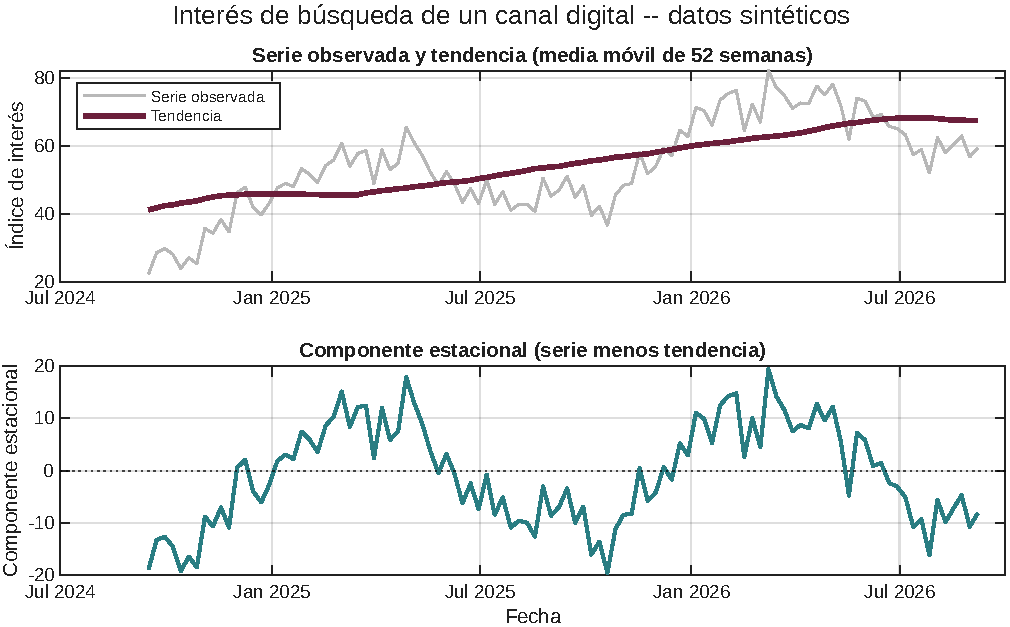
\includegraphics[width=0.95\textwidth]{figuras/matlab/cap04_tendencia_estacionalidad.pdf}
  \captionof{figure}{Serie de interés de búsqueda: observada, tendencia
  (media móvil de 52 semanas) y componente estacional. Fuente: elaboración
  propia con datos sintéticos, \texttt{rng(42)}.}
  \label{fig:cap04-tendencia}
\end{center}

\begin{center}
  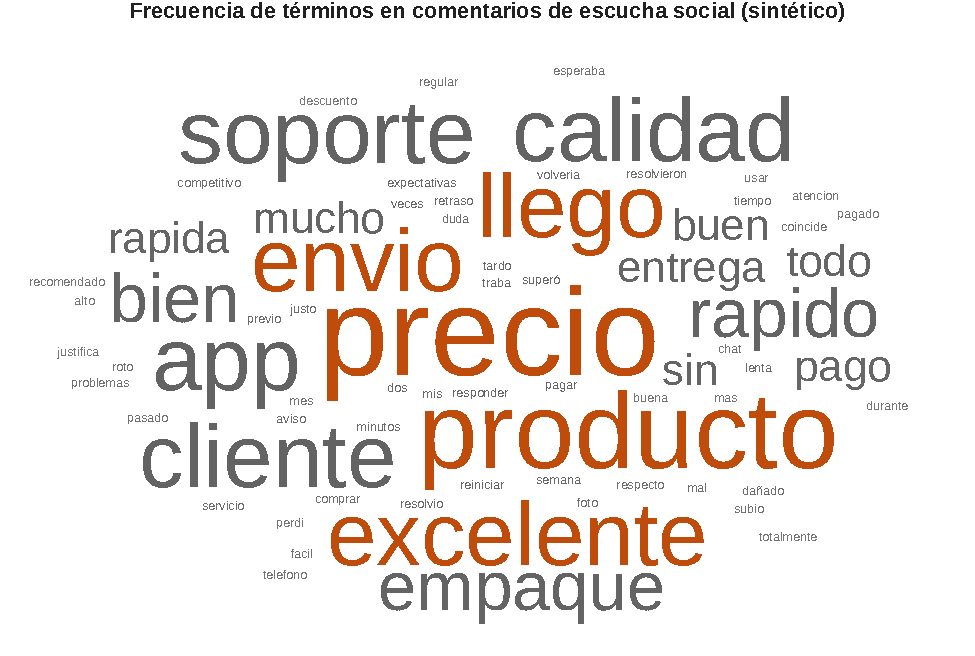
\includegraphics[width=0.72\textwidth]{figuras/matlab/cap04_nube_palabras.pdf}
  \captionof{figure}{Frecuencia de términos en un corpus sintético de
  escucha social. Fuente: elaboración propia con datos sintéticos.}
  \label{fig:cap04-nube}
\end{center}

\textbf{Interpretación de negocio.} El componente estacional de la
figura~\ref{fig:cap04-tendencia} (panel inferior) revela un patrón que la
serie observada (panel superior, línea gris) oculta a simple vista bajo el
ruido semana a semana: un pico recurrente hacia fin de año, de magnitud
similar en ambos ciclos anuales capturados. Una organización que planee
inventario, personal de soporte o presupuesto publicitario a partir de la
serie observada sin aislar este componente corre el riesgo de interpretar
como \enquote{tendencia acelerada} lo que en realidad es la fase ascendente
predecible del ciclo estacional —error que se repite cada fin de año en
organizaciones que no separan ambos componentes—. En la nube de palabras
(figura~\ref{fig:cap04-nube}), los términos dominantes —\textit{precio},
\textit{producto}, \textit{envío}, \textit{llegó}, \textit{excelente},
\textit{soporte}— mezclan menciones positivas y de fricción operativa a
simple vista indistinguibles por tamaño; el ejercicio propuesto pide separar
ambas.

\textbf{Ejercicio propuesto (usen exactamente este script, solo cambien el
bloque de parámetros).} Corran el script tres veces y completen un cuadro
con la amplitud estacional estimada y el valor máximo de la serie que
imprime cada corrida:
\begin{enumerate}
  \item \textbf{Caso A — valores por defecto:} los cuatro parámetros tal
  como están en el script.
  \item \textbf{Caso B — estacionalidad débil:} cambien
  \texttt{amplitudEstacional} de 12 a 3, sin tocar nada más.
  \item \textbf{Caso C — más ruido:} regresen \texttt{amplitudEstacional} a
  12 y cambien \texttt{desviacionRuido} de 4 a 15.
\end{enumerate}
Con el cuadro completo, respondan por escrito: en el Caso B, ¿el componente
estacional del panel inferior de la figura~\ref{fig:cap04-tendencia} sigue
siendo visible a simple vista en la serie observada (panel superior)? En el
Caso C, ¿la tendencia estimada por media móvil sigue viéndose suave, o el
ruido empieza a distorsionarla? A partir de sus tres corridas, expliquen en
qué condiciones (poco ruido y estacionalidad marcada, o mucho ruido y
estacionalidad débil) es más fácil confundir estacionalidad con tendencia en
un negocio real.

Como segunda parte del ejercicio, clasifiquen a mano los diez términos más
frecuentes del corpus de escucha social (fijo, no cambia entre corridas) en
\enquote{asociado a experiencia positiva}, \enquote{asociado a fricción
operativa} o \enquote{neutro/descriptivo}, y discutan si la nube de palabras,
por sí sola, sin ese trabajo manual de clasificación, es una herramienta de
análisis o solo de exploración inicial.

\textbf{Extensión opcional.} Sustituir la media móvil de 52 semanas por la
función \texttt{trenddecomp} o \texttt{decompose} disponible en el toolbox
de Econometría (si está instalado) y comparar el componente de tendencia
resultante contra el de este script.
\end{cajaLaboratorio}

\begin{cajaEtica}
Un corpus de escucha social real —a diferencia del sintético de este
laboratorio— contiene texto escrito por personas identificables o
potencialmente identificables. Analizarlo, incluso de forma agregada,
implica las mismas obligaciones de base legal revisadas en el Cap.~3: la
escucha social no está exenta de la LFPDPPP solo porque los comentarios sean
públicos. Publicar públicamente una opinión no equivale a otorgar
consentimiento ilimitado para cualquier uso analítico posterior de esa
opinión.
\end{cajaEtica}

\section{Estudio de caso}

\begin{casoFicticio}
El equipo de mercadotecnia de una marca de electrodomésticos mexicana
observa que su índice de interés de búsqueda de marca subió 20 puntos en
las últimas cuatro semanas y concluye que una campaña reciente de influencer
marketing está funcionando muy bien, con la intención de duplicar el
presupuesto de inmediato. Al revisar el histórico de dos años de la serie
—no solo las últimas cuatro semanas—, un analista nota que el mismo salto de
aproximadamente 20 puntos ocurrió en la misma época del año anterior, sin
ninguna campaña de influencers en curso en ese momento.

\textbf{Preguntas guía.}
\begin{enumerate}
  \item ¿Qué componente de la serie de tiempo (tendencia o estacionalidad)
  explica mejor el patrón que encontró el analista?
  \item Diseñe, en términos generales, cómo el equipo podría aislar el
  efecto real de la campaña de influencers del efecto estacional, usando el
  mismo enfoque de descomposición del laboratorio.
  \item ¿Qué consecuencia de negocio tendría duplicar el presupuesto de una
  campaña basándose en una lectura de la serie que confunde estacionalidad
  con efecto de campaña?
  \item Relacione este caso con la advertencia del caso de apertura sobre
  cifras puntuales de adopción tecnológica: ¿qué tienen en común el error de
  Gartner con el 25\,\% de caída de búsqueda y el error del equipo de
  mercadotecnia de este caso?
\end{enumerate}
\end{casoFicticio}

\section{Actividades y evidencias del portafolio}

\begin{description}
  \item[Reporte de indagación documental] Aplicar la matriz de cuatro
  criterios (cuadro~\ref{tab:cap04-criterios}) a dos plataformas digitales
  vigentes elegidas por el equipo, con al menos una fuente por criterio.
  \item[Exposición] Presentar el hallazgo del componente estacional del
  laboratorio (§3) y proponer una decisión de negocio distinta según se
  ignore o se considere ese componente.
  \item[Solución de casos] Resolver el estudio de caso de la marca de
  electrodomésticos (§4) por escrito.
  \item[Reporte de práctica] Consolidar, junto con el reporte de práctica
  del Cap.~3, el entregable único de la práctica oficial \enquote{Buscadores
  y plataformas en la gestión de datos del consumidor digital} (ver
  \enquote{Prácticas oficiales de la unidad} al cierre de esta Parte),
  incluyendo el cuadro de los tres casos del ejercicio propuesto del
  laboratorio (§3).
\end{description}

\section{Ruta de aprendizaje autónomo}

Una hora de aprendizaje autónomo. Tarea concreta:
\begin{enumerate}
  \item Investigar, con fecha de consulta registrada, si el estado del
  comercio agéntico descrito en el recuadro de Frontera de este capítulo
  (§2.1) cambió de forma relevante desde la fecha de cierre de este libro
  (18 de septiembre de 2026), y documentar la fuente.
\end{enumerate}

\section{Síntesis}

La base tecnológica del consumidor digital cambia más rápido que cualquier
libro de texto puede documentar con precisión permanente —el propio caso de
apertura de este capítulo lo demuestra con dos predicciones recientes que no
se cumplieron como se anunciaron—. La respuesta pedagógica correcta no es
memorizar el estado actual de las plataformas, sino dominar los criterios
que permiten evaluar cualquier plataforma, presente o futura: modelo de
negocio, intermediación de datos, interoperabilidad y exposición
regulatoria. Analíticamente, dos herramientas recorren todo el capítulo:
separar tendencia de estacionalidad en una serie de tiempo, y extraer
frecuencia de términos de un corpus de texto —ambas, técnicas que siguen
siendo válidas sin importar qué plataforma específica las alimente de
datos.

\subsection*{Glosario del capítulo}
\begin{description}
  \item[Amplitud estacional] Parámetro editable del script de este capítulo
  que controla qué tan marcado es el pico anual de la serie simulada. Rango:
  valor real $\geq 0$ (con 0, no hay componente estacional); los casos
  didácticos de este libro usan valores entre 3 y 12.
  \item[Bolsa de palabras (\textit{bag of words})] Representación de un
  corpus de texto como matriz de frecuencias de términos por documento.
  \item[Comercio agéntico] Comercio mediado por asistentes de compra basados
  en inteligencia artificial que buscan, comparan y en ocasiones ejecutan
  transacciones en nombre del consumidor.
  \item[Componente estacional] Patrón que se repite con periodicidad fija en
  una serie de tiempo (p.\,ej., anual).
  \item[Crecimiento semanal] Parámetro editable que controla la pendiente de
  la tendencia de la serie simulada (puntos de índice que suma cada semana).
  Rango: cualquier valor real; positivo para tendencia creciente, negativo
  para decreciente, cero para tendencia plana. El caso por defecto de este
  libro usa 0.35.
  \item[Desviación del ruido] Parámetro editable que controla la dispersión
  aleatoria semana a semana de la serie simulada. Rango: valor real $\geq 0$
  (con 0, la serie es perfectamente determinista); los casos didácticos de
  este libro usan valores entre 4 y 15.
  \item[Tendencia] Componente de cambio de largo plazo de una serie de
  tiempo, aislado del ruido de corto plazo y del patrón estacional.
\end{description}

\subsection*{Autoevaluación}

\textbf{Opción múltiple}

\begin{enumerate}
  \item El capítulo propone evaluar plataformas digitales con una matriz de
  criterios durables en vez de un catálogo de herramientas porque:
  \begin{enumerate}
    \item[a)] Las herramientas actuales son todas de mala calidad.
    \item[b)] Un catálogo de marcas concretas envejece más rápido que los criterios estructurales que las evalúan. \textit{(correcta)}
    \item[c)] El programa oficial prohíbe mencionar marcas.
    \item[d)] Las plataformas no tienen modelos de negocio distintos entre sí.
  \end{enumerate}
  \textit{Justificación:} §2.1.

  \item En la descomposición de una serie de tiempo, el componente
  estacional se obtiene, en el script del laboratorio, como:
  \begin{enumerate}
    \item[a)] La serie observada multiplicada por dos.
    \item[b)] La serie observada menos la tendencia estimada. \textit{(correcta)}
    \item[c)] El promedio simple de toda la serie.
    \item[d)] La frecuencia de términos del corpus de texto.
  \end{enumerate}
  \textit{Justificación:} §3, concepto detrás del código.
\end{enumerate}

\textbf{Preguntas abiertas}

\begin{enumerate}
  \item Explique por qué el capítulo no reporta cifras de cuota de mercado
  de buscadores ni de tamaño del comercio agéntico como datos verificados.
  \textit{Clave:} la respuesta debe señalar que las fuentes disponibles
  (blogs de industria, analistas) son de jerarquía baja y con frecuencia se
  contradicen entre sí, y que el criterio de verificación de datos de este
  libro exige no reportar como dato duro lo que no se puede confirmar en
  fuente primaria (§3 de este capítulo).
  \item Con base en el caso de apertura y el estudio de caso del capítulo,
  explique en sus propias palabras el riesgo de tomar decisiones de negocio
  a partir de una serie de tiempo sin separar tendencia, estacionalidad y
  ruido. \textit{Clave:} la respuesta debe identificar que confundir un
  patrón estacional recurrente con un efecto causal específico (una campaña,
  una predicción de mercado) lleva a decisiones de inversión mal
  fundamentadas, replicables en ambos casos presentados en el capítulo.
\end{enumerate}

\section{Lecturas recomendadas}

\begin{description}
  \item[\textcite{eprs2025darkpatterns}] Aunque centrado en patrones oscuros
  (desarrollado con detalle en el Cap. 7), este informe del Parlamento
  Europeo ofrece un panorama actualizado de regulación digital útil para el
  criterio de \enquote{exposición regulatoria} de la matriz de este
  capítulo.
  \item[\textcite{sheth2026}] Su enfoque de organizar el comportamiento
  digital por mecanismos de datos, más que por plataformas específicas, es
  coherente con el criterio metodológico que este capítulo propone para
  evaluar la base tecnológica.
\end{description}

% partes/parte1/practicas-oficiales.tex
\chapter*{Prácticas oficiales de la unidad — Parte I}
\addcontentsline{toc}{chapter}{Prácticas oficiales de la unidad — Parte I}

Esta sección consolida, con nombre y horas oficiales del programa, las dos
prácticas de la Unidad I. Los insumos de cada práctica ya se desarrollaron
en las secciones de laboratorio de los capítulos 1--4; aquí se presenta la
guía formal de entrega.

\textbf{Metodología común a ambas prácticas.} En los cuatro capítulos, el
laboratorio usa \textbf{el mismo script} que el estudiante entrega en su
práctica: no hay una versión \enquote{de clase} y otra \enquote{de tarea}
distintas. El script no se modifica más allá del bloque de parámetros,
claramente delimitado al inicio de cada archivo (\texttt{matlab/capNN/*.m}).
La tarea del estudiante es correr ese mismo script para dos o tres casos
distintos (cambiando solo datos o parámetros), registrar los resultados que
imprime y grafica cada corrida, compararlos entre sí y redactar una
conclusión propia. Ningún entregable requiere que el estudiante escriba o
edite código MATLAB más allá de sustituir valores en el bloque de
parámetros.

\section*{Práctica 1 — El consumidor digital y su perfil (7 h)}

\begin{description}
  \item[Capítulos que la integran] 1 y 2.
  \item[Lugar de realización] Aula / laboratorio.
  \item[Objetivo] Analizar la evolución y el perfil del consumidor digital
  aplicando, sobre distintos casos generados solo cambiando parámetros, el
  modelo de difusión de Bass (Cap.~1) y una segmentación rígida y difusa
  (Cap.~2).
  \item[Entregable] Reporte único que integre: (a) el cuadro de los tres
  casos del ejercicio propuesto del Cap.~1 (\texttt{cap01\_difusion\_bass.m},
  Casos A/B/C de innovación vs. imitación) con las dos preguntas de
  comparación respondidas; (b) el cuadro de los tres casos del ejercicio
  propuesto del Cap.~2 (\texttt{cap02\_segmentacion.m}, Casos A/B/C de
  traslape y número de arquetipos) con las tres preguntas de comparación
  respondidas; (c) una conclusión propia de media página que relacione ambos
  laboratorios con el concepto de perfil como función del negocio (Cap.~2,
  §2.5).
  \item[Criterios de evaluación] Los dos scripts se ejecutan sin modificar
  nada fuera del bloque de parámetros (verificable por reproducibilidad,
  \texttt{rng(42)}); los tres casos de cada script están completos, no solo
  el caso por defecto; interpretación de negocio propia, no copiada de este
  libro.
\end{description}

\section*{Práctica 2 — Buscadores y plataformas en la gestión de datos del consumidor digital (8 h)}

\begin{description}
  \item[Capítulos que la integran] 3 y 4.
  \item[Lugar de realización] Aula / laboratorio.
  \item[Objetivo] Aplicar limpieza de datos, segmentación RFM, CLV y prueba
  A/B (Cap.~3) junto con análisis de series de tiempo y frecuencia de
  términos (Cap.~4) para fundamentar una decisión de negocio digital, en
  cada caso comparando resultados entre corridas del mismo script.
  \item[Entregable] Reporte único que integre: (a) el cuadro de los tres
  casos del ejercicio propuesto del Cap.~3
  (\texttt{cap03\_rfm\_clv\_ab.m}, Casos A/B/C de tamaño de muestra y nivel
  de significancia de la prueba A/B) con las tres preguntas de comparación
  respondidas; (b) el cuadro de los tres casos del ejercicio propuesto del
  Cap.~4 (\texttt{cap04\_series\_texto.m}, Casos A/B/C de amplitud
  estacional y ruido) junto con la clasificación de los diez términos más
  frecuentes del corpus de escucha social; (c) aplicación de la matriz de
  cuatro criterios del Cap.~4 a una plataforma digital real elegida por el
  equipo.
  \item[Criterios de evaluación] Rigor estadístico en la prueba A/B (uso
  correcto del valor $p$, no solo comparación de porcentajes, y explicación
  de por qué el mismo par de proporciones puede cambiar de decisión al
  cambiar el tamaño de muestra); aplicación correcta y honesta de la matriz
  de criterios (sin promoción implícita de ninguna plataforma); todas las
  cifras de mercado citadas en el entregable deben tener fuente y fecha de
  consulta.
\end{description}


% --- PARTE II — V: se agregan en fases posteriores (§12) ---

\backmatter
\printbibliography
\printglossaries

\end{document}
